\chapter{Identify ambiguous tasks}
\label{chap:waum}

\enlargethispage{3\baselineskip}

\begin{keypointstwomargins}{Identify ambiguous tasks}{-2cm}{-1cm}

        \textbf{Key points -- Identify ambiguous tasks}
        \begin{enumerate}[leftmargin=*]
        \item We know that datasets with better quality will lead to better models. It is famously a complicated task to explore big datasets and find ambiguous tasks in a classical supervised setting. What can we do for crowdsourced datasets?
        \item While entropy or variance-based methods in distribution votes are useful to retrieve tasks that lead to very noisy decisions, they are not fit in settings with few votes per task. And even less fitted to settings where a task can be labeled by a single worker. Can we still exploit these tasks?
        \end{enumerate}

        \textbf{Contributions -- Weighted Area Under the Margin}
        \begin{enumerate}[leftmargin=*,start=3]
        \item Following the literature on label noise, we adapt the AUM by \citet{pleiss_identifying_2020} into the AUMC and WAUM, two strategies to identify ambiguous tasks in datasets. The first is the baseline and directly falls back to the classical AUM using a majority vote. The WAUM introduces a trust score in the balance not to use poorly performing workers' answers.
        \item We provide a simple guideline: pruning most ambiguous tasks from the dataset, and reporting computer vision classifier performance with and without pruning on simulated and three real datasets: \texttt{CIFAR-10H}, \texttt{LabelMe} and \texttt{Music}.
        \end{enumerate}

\end{keypointstwomargins}

\section{Do we know what is in our training sets?}
While our datasets are getting larger and larger every year, one question naturally arises: \emph{What is the quality of our training sets?}
Indeed, small datasets can easily be looked at, but thousands of images -- if not millions -- represent herculean human work without assistance.
Mistakes happen, and the quality of the data is not always perfect (\Cref{fig:label_mistakes}).

\begin{figure}[thb]
\centering
\begin{minipage}{.3\linewidth}
\centering
\subfloat[$y^\star=\texttt{cat}$ in CIFAR-10 \citep{krizhevsky2009learning}]{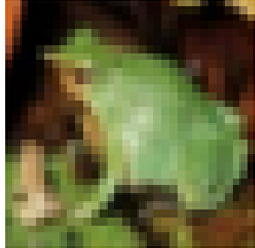
\includegraphics[width=\textwidth]{./chapters/images/catcifar.pdf}}
\end{minipage}%
\hfill
\begin{minipage}{.3\linewidth}
\centering
\subfloat[$y^\star=\texttt{tshirt}$ in Quickdraw]{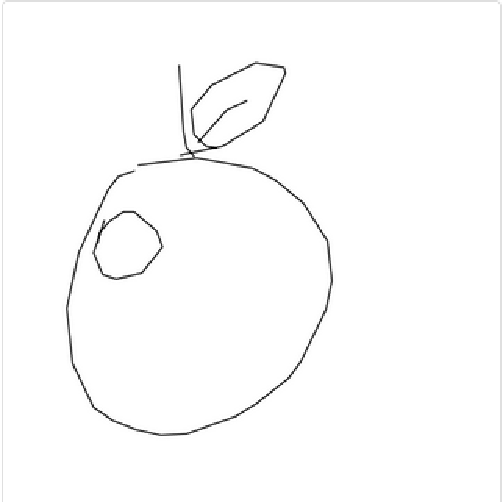
\includegraphics[width=\textwidth]{./chapters/images/tshirtquickdraw.pdf}}
\end{minipage}%
\hfill
\begin{minipage}{.3\linewidth}
\centering
\subfloat[$y^\star=\texttt{6}$ in MNIST \citep{deng2012mnist}]{
\includegraphics[width=\textwidth]{./chapters/images/6mnist.pdf}}
\end{minipage}
\caption{Three examples of labeling mistakes in classical classification datasets. The label can be wrong (CIFAR-10 and Quickdraw) or the task can be too ambiguous to classify (MNIST).}
\label{fig:label_mistakes}
\end{figure}


Data quality is linked with model performance \citep{budach2022effects}, looking for outliers to prune or weight differently during the learning procedure is not new \citep{angelova2004data}.
In this chapter, we first present the Area Under the Margin ($\AUM$): a statistic from \citet{pleiss_identifying_2020} that uses model iterates score prediction to detect unreliable training data points in the classically supervised learning setting.
Then, we propose to extend the $\AUM$ to the crowdsourcing setting with the Weighted Areas Under the Margin ($\WAUM$).
We show that the $\WAUM$ allows the identification of ambiguous tasks in crowdsourced datasets, and pruning a portion of those tasks leads to better test performance overall.

\subsection{Detect labeling errors in classical datasets}
% Cleanlab, confident learning, aum (litterature presentation and motivation mostly)
In classically supervised learning settings, training sets, tasks are paired up with a single label: $\mathcal{D}_\text{train}:=\{(x_i,y_i)\}_{i\in [n_\text{task}]}$.
This label has been assigned either automatically or via human decision.
Thus, the task might be mislabeled.
We can see a mislabeled task as a task that is difficult to classify for the classifier given this wrong label.
The $\AUM$ from \citet{pleiss_identifying_2020} allows us to identify tasks that are the most difficult to classify from the dataset.

More formally, the $\AUM$ of a task $(x_i,y_i)$ from a training set $\mathcal{D}_\text{train}$ given a classifier $\mathcal{C}$ and a number of training epochs $T>0$ is defined as:
\begin{equation}\label{eq:aum}
    \mathrm{AUM}\left(x, y; \mathcal{D}_{\texttt{train}}\right)
    = \!\! \frac{1}{T}\sum_{t=1}^T \!\! \big[\sigma^{(t)}_{y} (x)- \sigma^{(t)}_{[2]}(x)\big]
    \enspace.
\end{equation}
The $\AUM$ averages over time how far the score for the given class is from the most predicted other class by the classifier.
This is an average over time of the prediction margin.
It is classic to look at this margin in the literature to bound test error.
For example, \citet{bartlett1998boosting} showed that test error is dependent on the margin's distribution over the training set, even with zero error reached during training.
However, the $\AUM$ does not consider the margin given a trained classifier but looks at the early dynamics in the training procedure.
\citet{pleiss_identifying_2020} use an average of margins over logit scores, while we rather consider the average of margin after a softmax step in \Cref{eq:aum},
% Indeed, the original $\mathrm{AUM}$ relies on logit scores by applying a $\softmax$ step.
to temper scaling issues, as advocated by \citet{ju2018relative} in ensemble learning.
Moreover, we consider the margin introduced by \citet{yang2020consistency} since the corresponding hinge loss has better theoretical properties than the one used in the original $\mathrm{AUM}$, especially in top-$k$ settings\footnote{For top-$k$, consider $\sigma^{(t)}_{[k+1]}(x)$ instead of $\sigma^{(t)}_{[2]}(x)$ in \eqref{eq:aum}.} \citep{lapin2016loss, yang2020consistency,Garcin_Servajean_Joly_Salmon22}. However, one could easily consider the original margin with few differences in practice for top-$1$ classification. The algorithm to compute the $\mathrm{AUM}$ is detailed in \Cref{alg:AUM}.

\begin{figure}[thb]
\begin{minipage}{.45\linewidth}
\centering
\subfloat[Mislabeled image: $\AUM\ll 0$]{\label{mnist:low}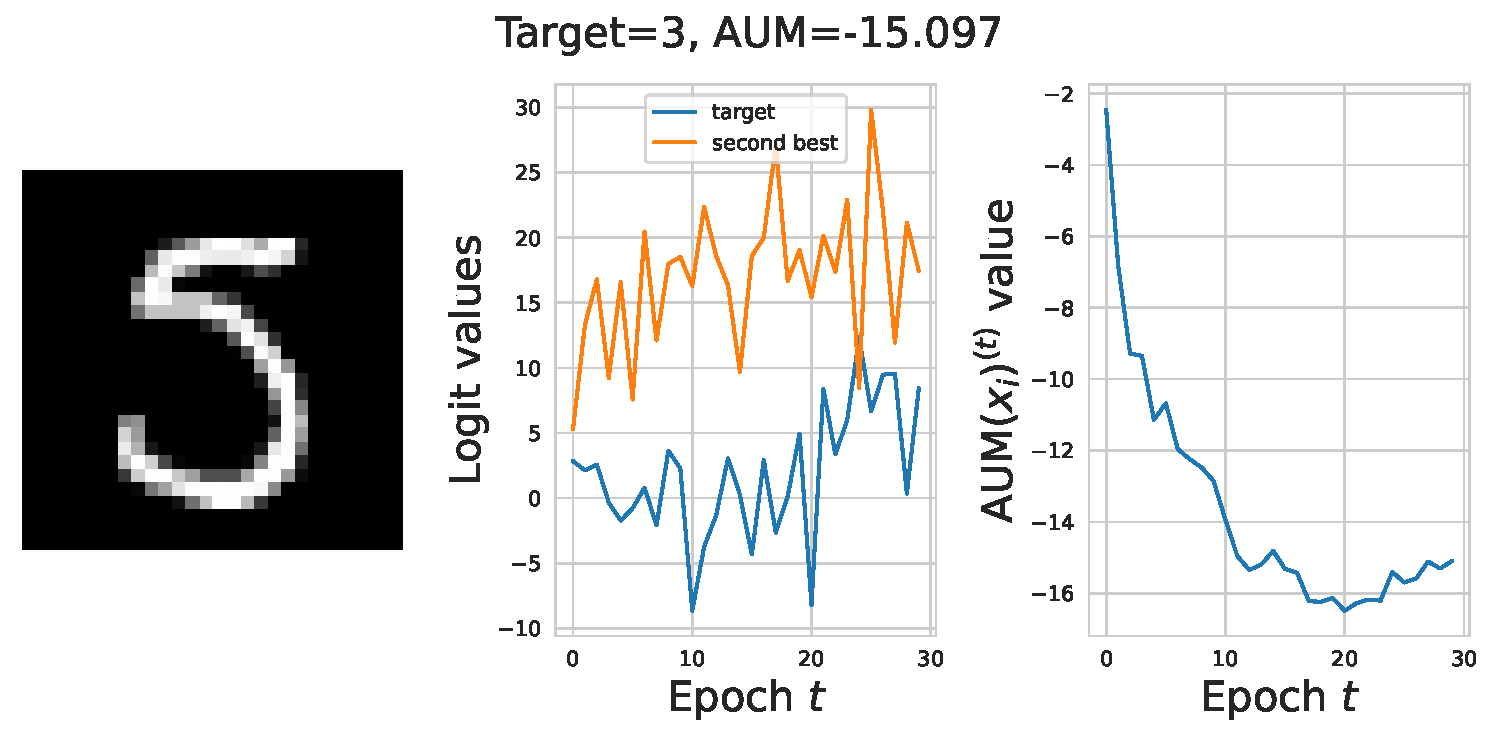
\includegraphics[width=\textwidth]{chapters/images/low_aum_mnist.pdf}}
\end{minipage}%
\hfill
\begin{minipage}{.45\linewidth}
\centering
\subfloat[Correct label: $\AUM\gg 0$]{\label{mnist:high}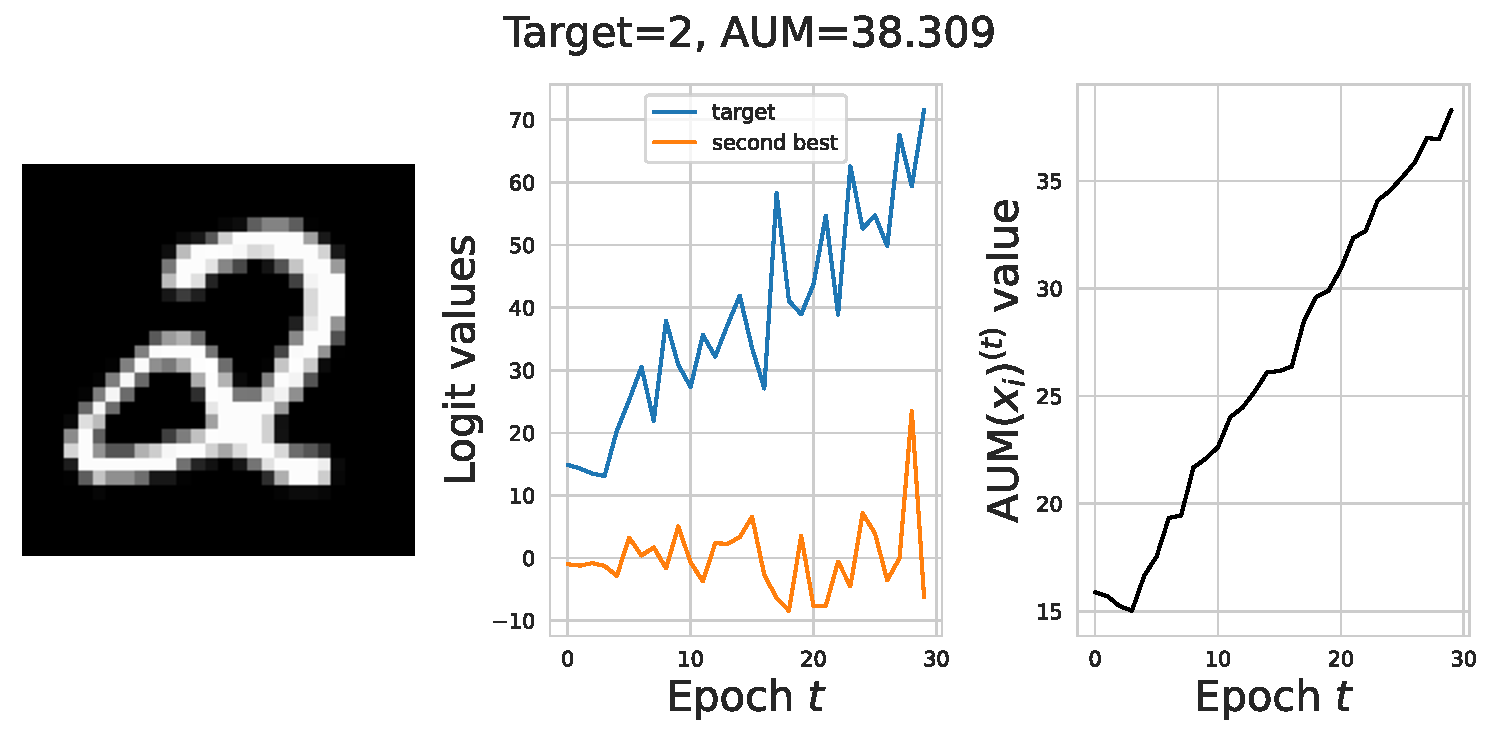
\includegraphics[width=\textwidth]{chapters/images/high_aum_mnist.pdf}}
\end{minipage}\par\medskip
\begin{center}
\subfloat[Confusion: the image is either a four or a nine cut-out with true label $y_i^\star=9$, the $\AUM$ is closer to zero indicating high ambiguity in learning classes]{\label{mnist:mid}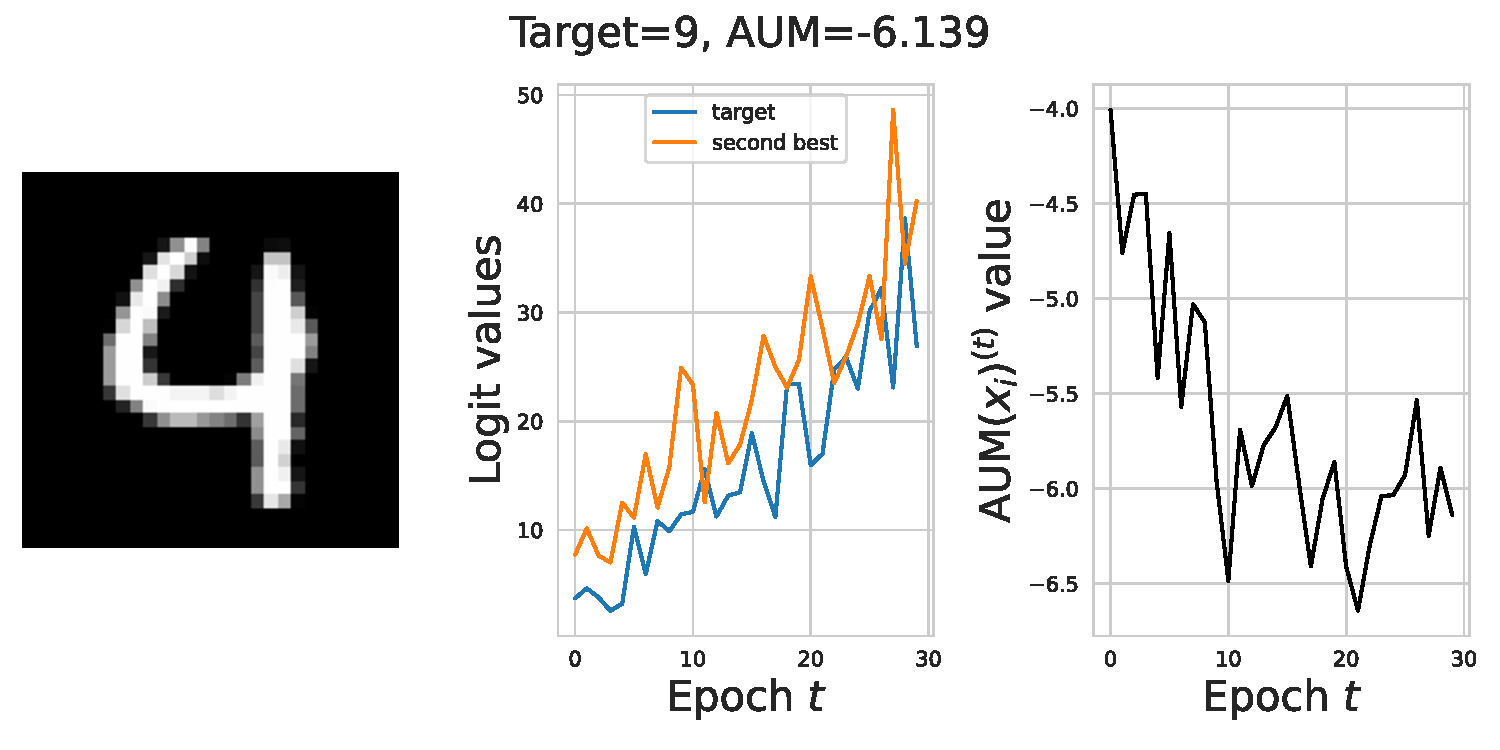
\includegraphics[width=.6\textwidth]{chapters/images/mid_aum_mnist.pdf}}
\end{center}
\caption{Three examples from the MNIST dataset to illustrate the behavior of the $\AUM$: if the sample is mislabeled the $\AUM$ is low as the classifier disagrees with the given label. Note that if $T>0$ is too high the memorization kicks in and the $\AUM$ increases again. When the sample is correctly labeled the $\AUM$ increases over training. When the sample is ambiguous, the $\AUM$ is closer to $0$. Results are from a 2-layer convolution network with max-pooling. Training is done in $T=30$ epochs using Adam optimizer with a learning rate set to $0.01$ and batches of $100$ samples.}
\label{fig:mnist_aum}
\end{figure}

This early dynamic, and by association the hyperparameter $T>0$, is necessary as it is well known that modern neural networks classifiers can memorize the data and even classify correctly random tasks because of the hyperparametrization \citep{maennel2020neural}.
Memorization is a necessary phenomenon for training a neural network: we need the classifier to memorize patterns.
But what we wish to consider the least in the $\AUM$ is the unintended memorization \citep{maennel2020neural} that can happen early and is difficult to temper -- even with strategies like dropout or weight decay.
And in \citet{zhang2021understanding}, they show -- among other results -- that true labels are learned faster than random labels by neural networks classifier.
This early training dynamic in the prediction logits can thus be used as a proxy to identify possible mislabeled data.

Note that there exist other algorithms to learn from mislabeled data, such as Confident Learning \citep{northcutt_confident_2021} using by \texttt{CleanLab}\footnote{\url{https://cleanlab.ai/}}.
Confident Learning does not correct the label nor does it re-weight the data.
It estimates the joint distribution between the given and unknown latent labels with class-conditional noise and then prunes samples by class with a threshold of the average predicted probability for the samples in the given class.
With the $\AUM$, we can also correct the label during training -- even though we will not consider this application for this work.

We recall in \Cref{alg:AUM} how to compute the $\mathrm{AUM}$ in practice for a given training set $\mathcal{D}_{\text{train}}$.
This step is used within the $\mathrm{WAUM}$ (label aggregation step).
Overall, considering a model, computing the $\mathrm{AUM}$ requires an additional cost: $T$ training epochs are needed to record the margins' evolution for each task.
This usually represents less than twice the original time budget.
We recall that $\sigma^{(t)}(x_i)$ is the softmax output of the predicted scores for the task $x_i$ at iteration $t$.

\begin{algorithm}[htb]
    \caption{$\mathrm{AUM}$ algorithm}\label{alg:AUM}
    \begin{algorithmic}
    \STATE \textbf{Input:} $\mathcal{D}_{\text{train}}=(x_i, y_i)_{i\in[n_\texttt{task}]}$: training set with $n_\texttt{task}$ task/label couples, $T\in \mathbb{N}$: number of epochs
    \FOR{$t=1,\dots,T$}
    \STATE \textbf{Train} the neural network for the $t^{th}$ epoch, using $\mathcal{D}_{\text{train}}$\;
    \FOR{$i \in [n_{\texttt{task}}]$}
    \STATE\textbf{Record softmax} output $\sigma^{(t)}(x_i)\in\Delta_{K-1}$\;
    \STATE\textbf{Compute margin} $M^{(t)}(x_i, y_i)=\sigma^{(t)}_{y_i}(x_i) - \sigma^{(t)}_{[2]}(x_i)$\;
    \ENDFOR
    \ENDFOR
    \STATE $\forall i\in[n_{\texttt{task}}],\ \mathrm{AUM}(x_i, y_i;\mathcal{D}_{\text{train}})=\frac{1}{T}\sum_{t\in[T]}M^{(t)}(x_i, y_i)$
\end{algorithmic}
\end{algorithm}

\section{The WAUM: extending the AUM to the crowdsourcing setting}

In this work, we aim at identifying ambiguous tasks from their associated features, hence discarding hurtful tasks (such as the ones illustrated on \Cref{fig:votes-c10h}) following the pipeline presented in \Cref{fig:crowdsourcing_scheme}. First, we collect the crowdsourced labels, then identify ambiguous tasks and prune them, and finally train a classifier on the pruned dataset.

\begin{figure}[thb]
    \centering
    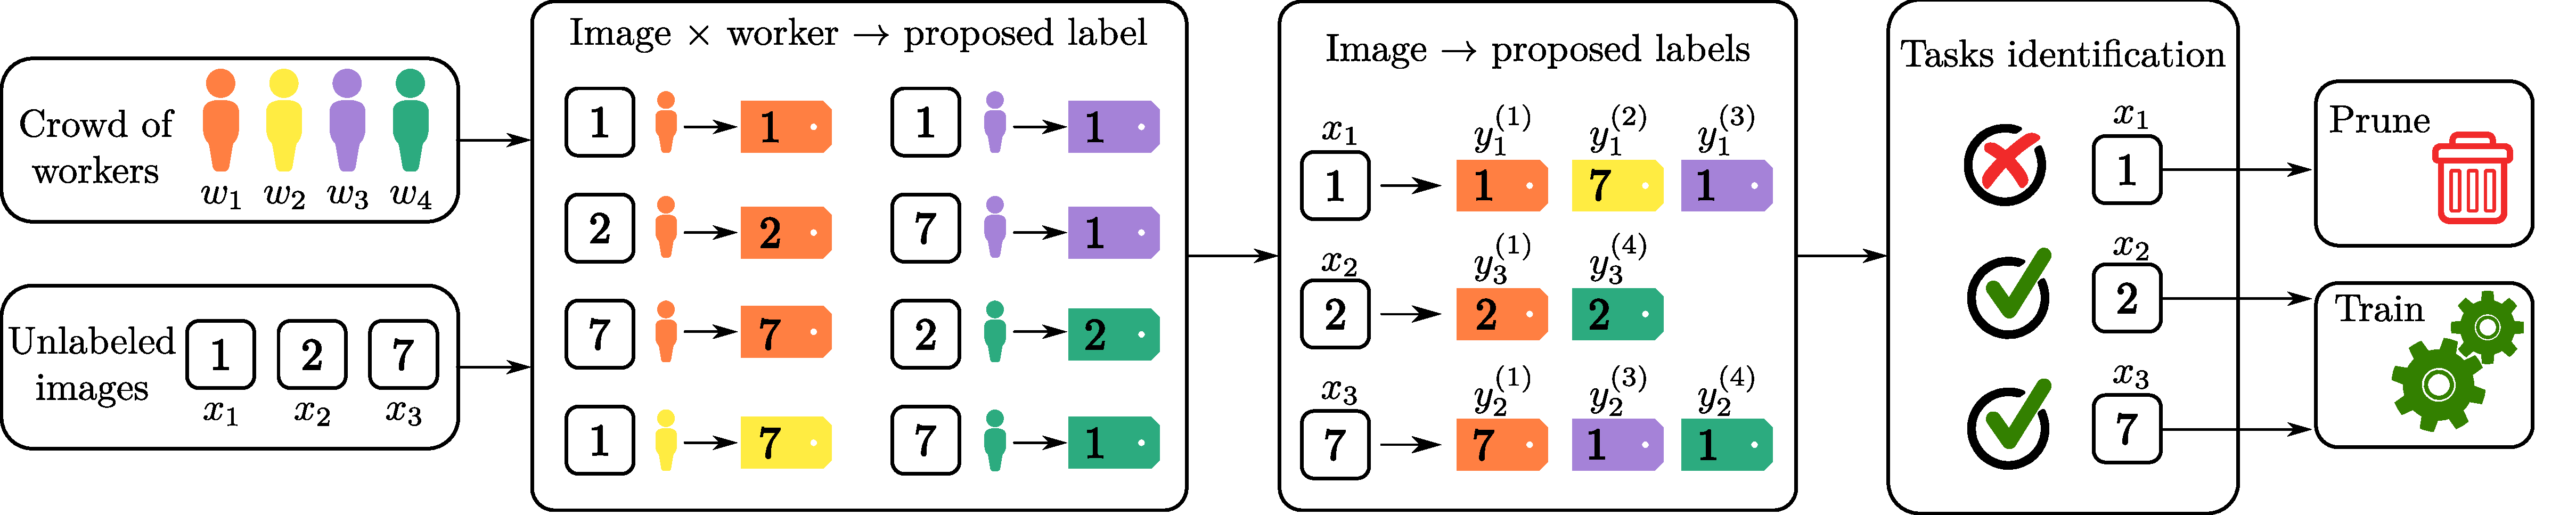
\includegraphics[width=.9\textwidth]{images/schema_crowdsourcing_en_with_notation_times}
    \caption{Learning with crowdsourcing labels: from label collection with a crowd to training on a pruned dataset. High ambiguity from either crowd workers or tasks intrinsic difficulty can lead to mislabeled data and harm generalization performance. To illustrate our notation, here the set of tasks annotated by worker $w_3$ is $\mathcal{T}(w_3)=\{1,3\}$ while the set of workers annotating task $x_3$ is $\mathcal{A}(x_3)=\{1,3,4\}$.}
    \label{fig:crowdsourcing_scheme}
\end{figure}

Recent works on data-cleaning in supervised learning \citep{han2019deep, pleiss_identifying_2020, northcutt_confident_2021} have shown that some images might be too corrupted or too ambiguous to be labeled by humans.
Hence, one should not consider these tasks for label aggregation or learning since they might reduce generalization power; see for instance \citep{pleiss_identifying_2020}.
Throughout this work, we consider the ambiguity of a task with the informal definition proposed by \citet{angelova2004data} that fit standard learning frameworks: \emph{``Difficult examples are those which obstruct the learning process or mislead the learning algorithm or those which are impossible to reconcile with the rest of the examples''}.
This definition links back to how \citet{pleiss_identifying_2020} detects corrupted samples using the area under the margin (AUM) during the training steps of a machine learning classifier.
However, it is important to notice that, in this context, the task ambiguity is inherent to the classifier architecture, and thus might not exactly overlap with human-level difficulty.

\begin{figure}[thb]
    \centering
    \begin{minipage}{.3\linewidth}
    \centering
    \subfloat[Label \texttt{deer} is meaningless here, and workers are confused with all other labels.]{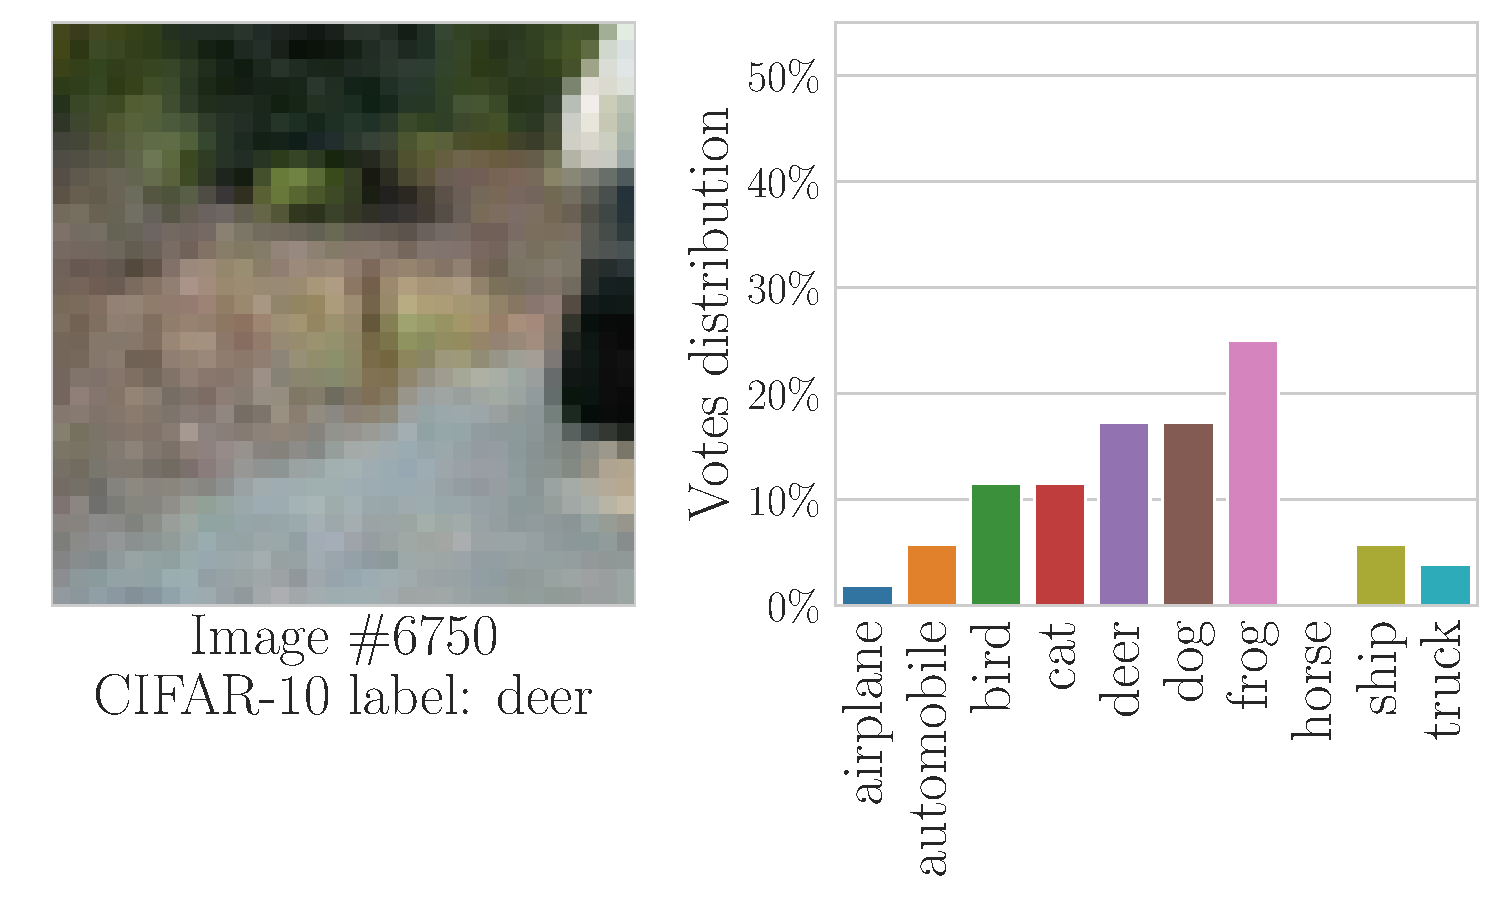
\includegraphics[width=\textwidth]{./chapters/images/image_n_hist6750_paper.pdf}}
    \end{minipage}%
    \hfill
    \begin{minipage}{.3\linewidth}
    \centering
    \subfloat[Label \texttt{airplane} is easy to identify (unanimity among workers).]{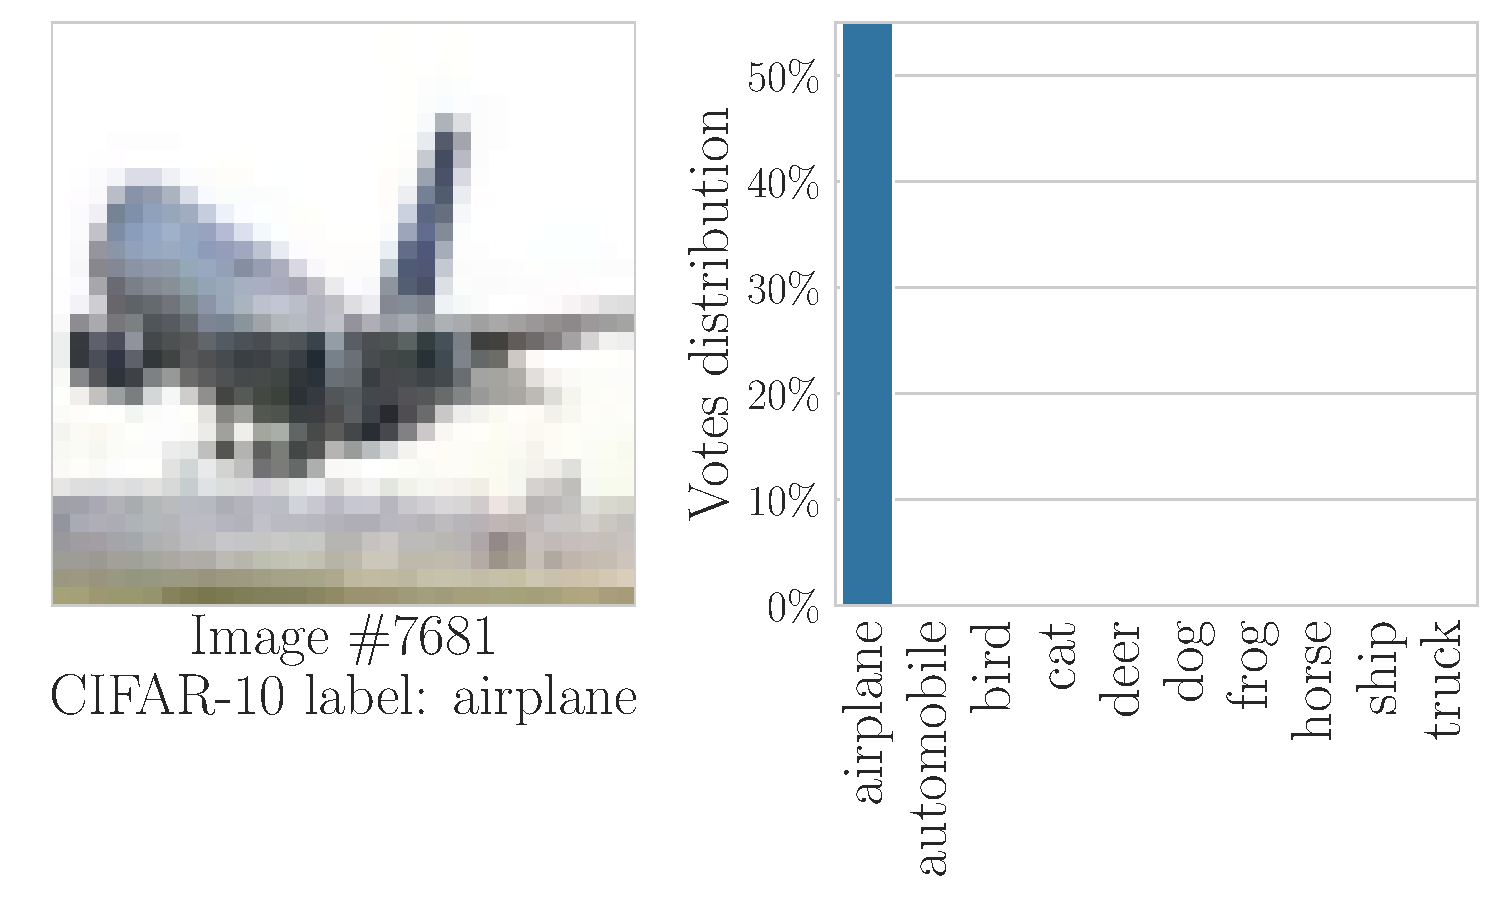
\includegraphics[width=\textwidth]{./chapters/images/image_n_hist7681_paper.pdf}}
    \end{minipage}%
    \hfill
    \begin{minipage}{.3\linewidth}
    \centering
    \subfloat[Label \texttt{cat} often confused with horns of a wild \texttt{deer}]{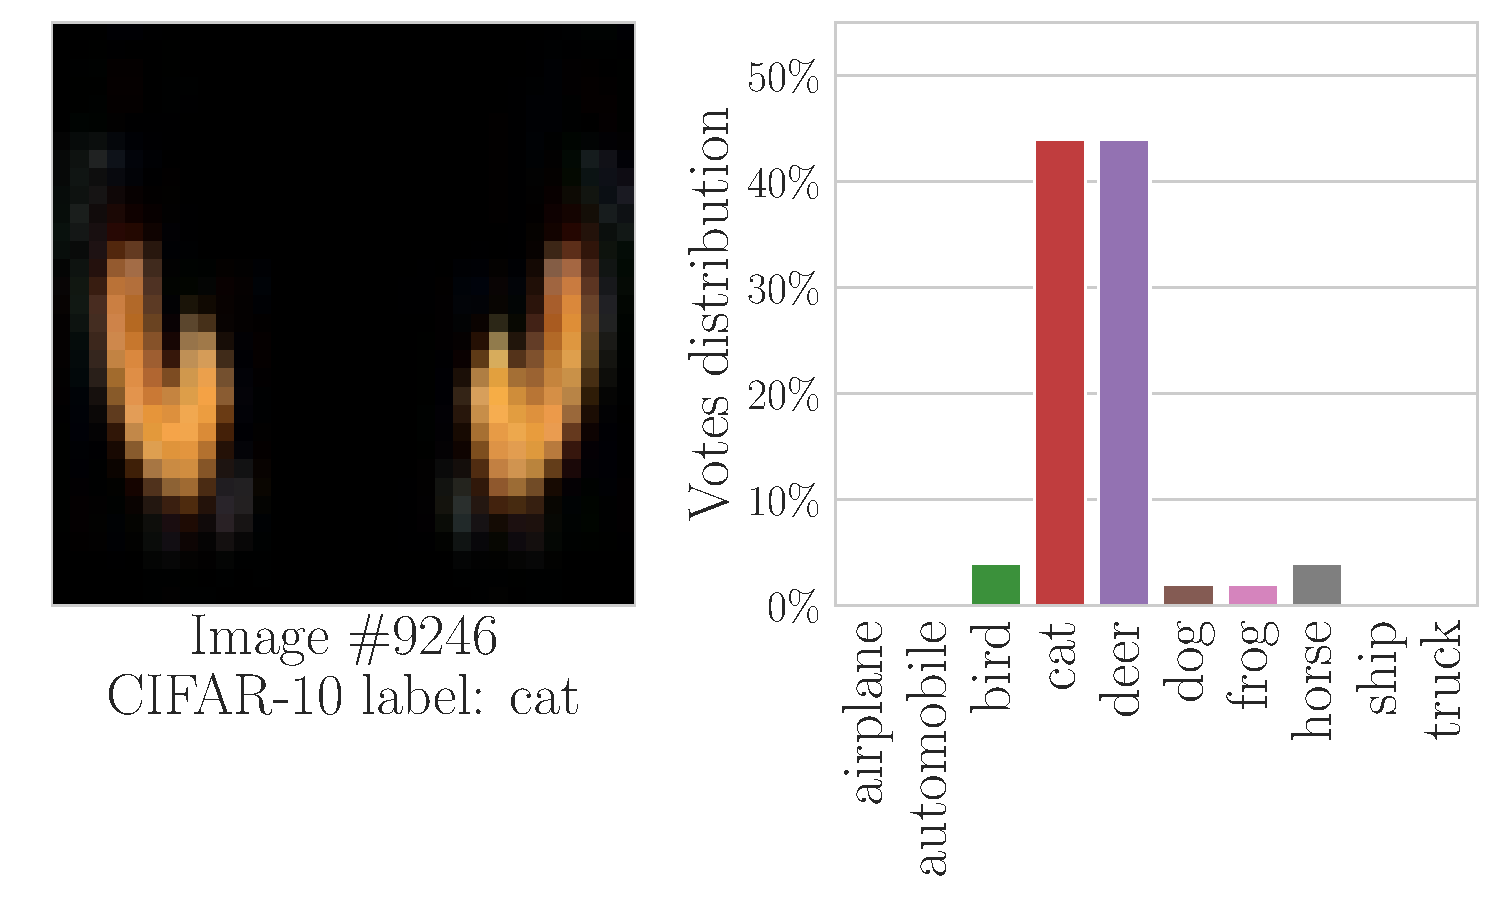
\includegraphics[width=\textwidth]{./chapters/images/image_n_hist9246_paper.pdf}}
    \end{minipage}
    \caption{Three images from \texttt{CIFAR-10H} dataset \citep{peterson_human_2019}, with the empirical distribution of workers' labels (soft labels): the \texttt{airplane} image (a) is easy, while the landscape (b) is ambiguous due to the image's poor quality. The last image (c) looks like a black cat face often perceived as the horns of a \texttt{deer}.}
    \label{fig:votes-c10h}
    \end{figure}

While the $\AUM$ shows results of identifying different types of sample difficulty by averaging the margin during $T>0$ training epochs, there is no direct way to apply it to the crowdsourcing setting.
Indeed, the $\AUM$ needs, by definition, a hard label $y_i$ to consider the assigned-label score $\mathcal{C}(x_i)_{y_i}$ and also to consider the second biggest score for a class different than $y_i$.
In the crowdsourcing setting however, there is no direct hard label $\hat y_i$ from the multiple answers $\{y_i^{(j)}\}_{j\in\mathcal{A}(x_i)}$ to a task $x_i$.


A naive transformation to apply the $\AUM$ in a crowdsourcing setting is to consider the majority voting aggregation. \Cref{eq:aum} simply becomes:
\begin{equation}\label{eq:aum_mv}
    \mathrm{AUMC}\left(x_i,\left\{y_i^{(j)}\right\}_{j\in\mathcal{A}(x_i)};\mathcal{D}_\texttt{train}\right) = \frac{1}{T}\sum_{t=1}^T \left[\sigma_{\hat y_i^{\mathrm{MV}}}^{(t)}(x_i) - \sigma_{[2]}^{(t)}(x_i)\right] \enspace.
\end{equation}
The $\AUM\mathrm{C}$ strategy lacks the worker abilities and task difficulty.
There is no worker-specific margin, the MV aggregation strategy removed the worker-specific information from the $\AUM$.
In the following, we introduce the $\WAUM$: a statistic that generalizes the $\AUM$ to the crowdsourcing setting by aggregating worker-specific margins into a weighted average to consider both worker abilities and task difficulty.

\subsubsection{Out-of-Model-Scope and task difficulty.}
Identifying ambiguous tasks in a training set seems close to the Out-Of-Distribution (OOD) detection problem -- when we aim at detecting data that is not from the same distribution as our training set \citep{schorn2020facer,wang2022vim}.
Given a new data point, a monitoring system is built to detect if that point comes from the same distribution as the data used to train a model or whether it deviates significantly from that distribution.
Similarly, recent works argue that the Out-Of-Model-Scope (OMS) detection problem is a more general problem than OOD detection \citep{granese2021doctor,guerin2023out}.
Given a model, we construct its scope as the set of data where the model is correct.
A monitor is built so that, given a new task, we can detect if the model is suited or not to classify it.
It is a model-dependent problem, and the scope is defined by the model's architecture and training data, contrary to the OOD problem which is only dependent on the training data.

However, both the OOD and the OMS detection problems are not the same as identifying ambiguous tasks in our setting.
Indeed, OOD detection relies on testing whether the task is from the same distribution as the training set without a network.
The OMS detection relies on testing whether the task is in the trained model scope at evaluation time.
We consider with the $\AUM$, and the $\WAUM$, the task difficulty in the training set, given a new model, how to identify ambiguous tasks before the evaluation step.

\subsection{Definition and construction of the WAUM}
\label{sub:def_waum}
% Explain weights choice and variations

We thus introduce the Weighted Area Under the Margin ($\mathrm{WAUM}$), a generalization to the crowdsourcing setting of the Area Under the Margin ($\mathrm{AUM}$) by \citet{pleiss_identifying_2020}.
We essentially combine task difficulty scores with worker abilities scores, but we measure the task difficulty by incorporating feature information.
The $\mathrm{AUM}$ is a confidence indicator in an assigned label defined for each training task.
It is computed as an average of margins over scores obtained along the learning steps.
The $\mathrm{AUM}$ reflects how a learning procedure struggles to classify a task to an assigned label.
The $\mathrm{AUM}$ is well suited when training a neural network (where the steps are training epochs) or other iterative methods.
For instance, it has led to better network calibration \citep{park2022calibration} using MixUp strategy \citep{zhang2017mixup}, \emph{i.e.} mixing tasks identified as simple and difficult by the $\mathrm{AUM}$.
The $\mathrm{WAUM}$, our extension of the $\mathrm{AUM}$, aims at identifying ambiguous data points in crowdsourced datasets, so one can prune ambiguous tasks that degrade the generalization.
It is a weighted average of workers $\mathrm{AUM}$, where the weights reflect trust scores based on task difficulty and workers' ability.

Given several training epochs $T>0$ and a classifier $\mathcal{C}$ for a crowdsourced training set $\mathcal{D}_\text{train}$, we write the $\WAUM$ as a weighted average of worker specific $\AUM$.
Let $s^{(j)}(x_i)\in [0,1]$ be a trust factor in the answer of worker $w_j$ for task $x_i$.
The $\mathrm{WAUM}$ is then defined as:
\begin{align}
    \label{eq:WAUM}
    \mathrm{WAUM}(x_i)
     &
    = \tfrac{
    \displaystyle \sum_{j\in\mathcal{A}(x_i)}  \!\!\!
    s^{(j)}(x_i) \mathrm{AUM}\big(x_i, y_i^{(j)}\big)
    }
    {\displaystyle\sum_{j'\in\mathcal{A}(x_i)}
    s^{(j')}(x_i)}
    \enspace.
\end{align}
It is a weighted average of $\mathrm{AUM}$s over each worker's answer with a per task weighting score $s^{(j)}(x_i)$ based on workers' abilities.
This score considers the impact of the $\mathrm{AUM}$ for each answer since it is more informative if the $\mathrm{AUM}$ indicates uncertainty for an expert than for a non-expert.


The scores $s^{(j)}$ are obtained \emph{à la} \citet{servajean2017crowdsourcing}: each worker has an estimated confusion matrix $\hat{\pi}^{(j)}\in \mathbb{R}^{K\times K}$.
Note that the vector $\mathrm{diag}(\hat{\pi}^{(j)}) \in \mathbb{R}^{K}$ represents the probability for worker $w_j$ to answer correctly to each label.
With a neural network classifier, we estimate the probability for the input $x_i\in\mathcal{X}_\texttt{train} $ to belong in each category by $\smash{\sigma^{(T)}(x_i)}$, \emph{i.e.} the probability estimate at the last epoch.
As a trust factor, we propose the inner product between the diagonal of the confusion matrix and the softmax vector:
\begin{align}\label{eq:trust_factor}
    s^{(j)}(x_i) = \big\langle \mathrm{diag}(\hat{\pi}^{(j)}) , \sigma^{(T)}(x_i) \big\rangle \in [0,1] \enspace.
\end{align}
The scores control the weight of each worker in \Cref{eq:WAUM}.
This choice of weight is inspired by the bilinear scoring system of $\mathrm{GLAD}$ \citep{whitehill_whose_2009}, as detailed hereafter.
The closer to one, the more we trust the worker for the given task.
The score $s^{(j)}(x_i)$ can be seen as a multidimensional version of $\mathrm{GLAD}$'s trust score.
Indeed, in  $\mathrm{GLAD}$, the trust score is modeled as the product $\alpha_j\beta_i$, with $\alpha_j\in\mathbb{R}$ (resp. $\beta_i\in (0, +\infty)$) representing worker ability (resp. task difficulty).
In \Cref{eq:trust_factor}, the diagonal of the confusion matrix $\hat{\pi}^{(j)}$ represents the worker's ability and the softmax the task difficulty.

\begin{constructionbox}[Construction of the WAUM]
    Given a single task $x_i$ and a worker $w_j\in\mathcal{A}(x_i)$, a possible measure of label ambiguity is the $\mathrm{AUM}$:
    \begin{equation*}
        \mathrm{AUM}\big(x_i, y_i^{(j)}\big) = \frac{1}{T}\sum_{t=1}^T \big[\sigma^{(t)}_{y_i^{(j)}}(x_i) - \sigma^{(t)}_{[2]}(x_i)\big] \enspace.
    \end{equation*}
    Extending to multiple workers $(w_j)_{j\in\mathcal{A}(x_i)}$, a naive extension (other than the $\mathrm{AUMC}$) would be to average the $\mathrm{AUM}$ over workers:
    \begin{equation*}
        \widetilde{\mathrm{WAUM}}\big(x_i, \{y_i^{(j)}\}_j\big) = \frac{1}{|\mathcal{A}(x_i)|}\sum_{j\in\mathcal{A}(x_i)}\left[\frac{1}{T}\sum_{t=1}^T \big[\sigma^{(t)}_{y_i^{(j)}}(x_i) - \sigma^{(t)}_{[2]}(x_i)\big]\right] \enspace.
    \end{equation*}
    However, by doing so the averaged ambiguity does not consider the worker performance. If the worker performs poorly, they should not contribute much to the overall task ambiguity. Hence the proposition is to use a weight $s^{(j)}(x_i)$ that considers both the worker and the task. Instead of the classical average, we thus obtain the weighted average defined in \Cref{eq:WAUM}.
    \end{constructionbox}


\subsubsection{Why variance or entropy-based identifications are not always suited.}

The natural choice instead of the $\mathrm{WAUM}$ would be to use the entropy of the votes to detect ambiguous tasks. However, the entropy of the votes is not always suited for difficulty identification.
Indeed, when large amounts of votes per task are available, the entropy of the votes and the $\mathrm{WAUM}$ coincide well, as in \Cref{fig:entropy_vs_waum}(a).
Yet, when votes are scarce, as in \Cref{fig:entropy_vs_waum}(b) and (c), entropy becomes irrelevant while our introduced $\mathrm{WAUM}$ remains useful.

\begin{figure}[thb]
    \centering
    \hfill
    \subfloat[\texttt{CIFAR-10H} dataset.]{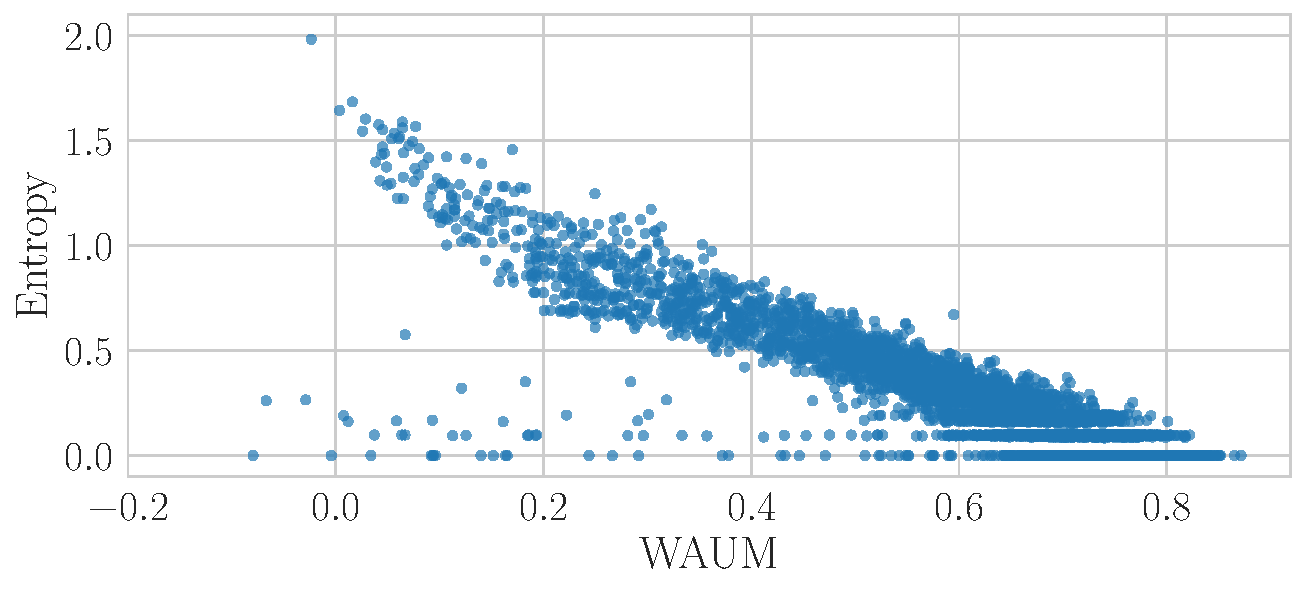
\includegraphics[width=0.3083\textwidth]{images/scatter_entropy_vs_waum_CIFAR-10H.pdf}}
    \hfill
    \subfloat[\texttt{LabelMe} dataset.]{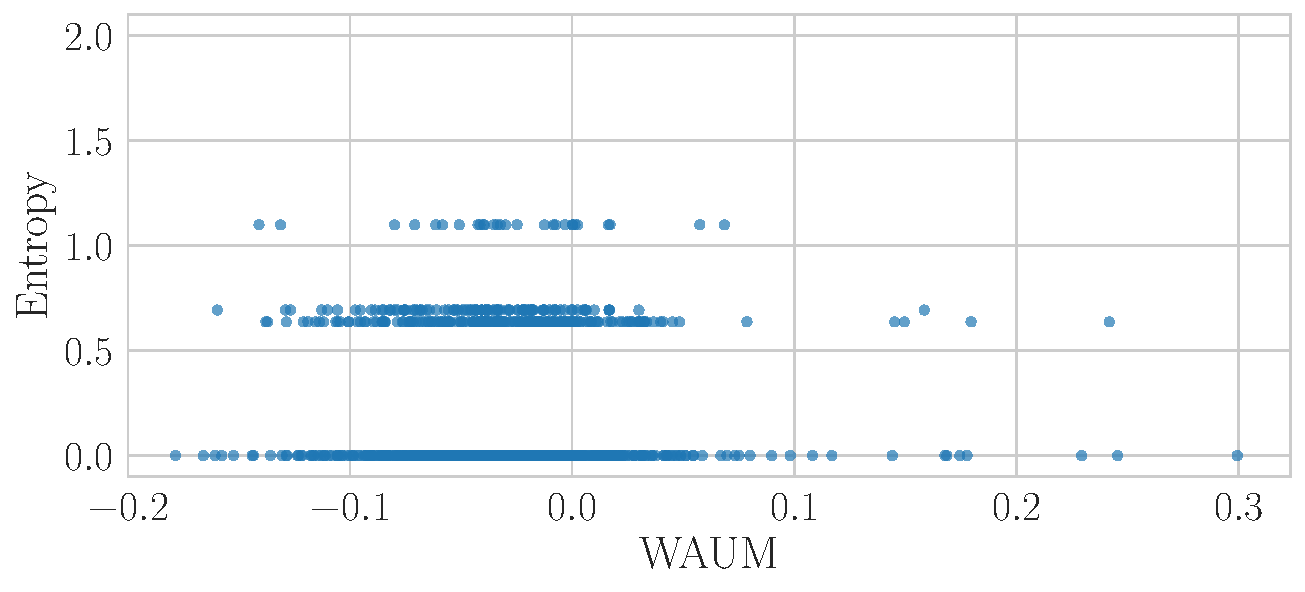
\includegraphics[width=0.3083\textwidth]{images/scatter_entropy_vs_waum_LabelMe}}
    \hfill
    \subfloat[\texttt{Music} dataset.]{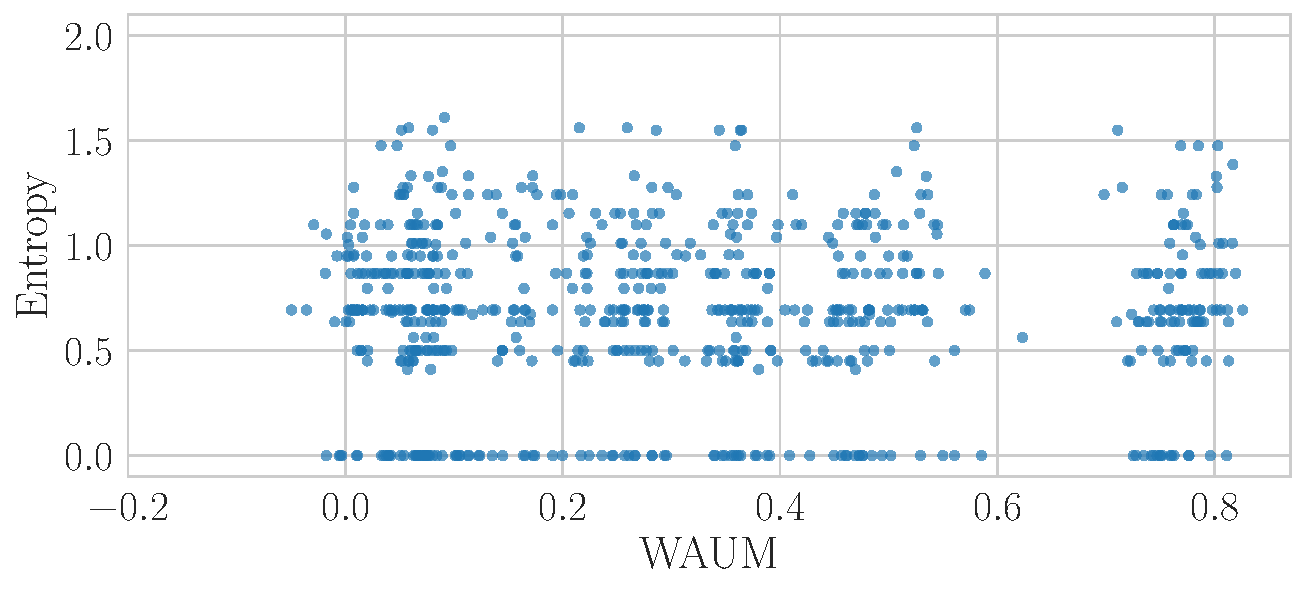
\includegraphics[width=0.3083\textwidth]{images/scatter_entropy_vs_waum_Music}}
    \hfill
    \caption{Entropy of votes vs. $\mathrm{WAUM}$ for \texttt{CIFAR-10H}, \texttt{LabelMe}, and \texttt{Music}, each point representing a task/image. When large amounts of votes per task are available, $\mathrm{WAUM}$ and entropy ranking coincide well, as in (a). Yet, when votes are scarce, as in (b) and (c), entropy becomes irrelevant while our introduced $\mathrm{WAUM}$ remains useful. Indeed, tasks with few votes can benefit from feedback obtained for a similar one. And for the \texttt{LabelMe} dataset in particular, there are only up to three votes available per task, thus only four different values of the entropy possible, making it irrelevant in such cases for modeling task difficulty.}
    \label{fig:entropy_vs_waum}%
\end{figure}

\subsubsection{Dataset Pruning and hyperparameter tuning.} Our procedure (\Cref{alg:WAUMstack}) proceeds as follows.
We initialize our method by estimating the confusion matrices for all workers.
For each worker $w_j$, the $\mathrm{AUM}$ is computed for its labeled tasks, and so is its worker-dependent trust scores $s^{(j)}(x_i)$ with \Cref{eq:trust_factor} during the training phase of a classifier.
The $\mathrm{WAUM}$ in \Cref{eq:WAUM} is then computed for each task.
The most ambiguous tasks, the ones whose $\mathrm{WAUM}$ are below a threshold, are then discarded, and the associated pruned dataset $\mathcal{D}_{\text{pruned}}$ is output. We consider for the pruning threshold a quantile of order $\alpha\in[0,1]$ of the $\mathrm{WAUM}$ scores.
The hyperparameter $\alpha$ (proportion of training data points pruned) can be chosen on a validation set, yet choosing $\alpha\in\{0.1, 0.05, 0.01\}$ has led to satisfactory results in all our experiments.
Note that the same pruning procedure can be applied to $\mathrm{AUMC}$ for comparison.
Both the $\mathrm{AUMC}$ and $\mathrm{WAUM}$ inherit the hyperparameter $T>0$ from the original $\mathrm{AUM}$.
Following the recommendations from \citet{pleiss_identifying_2020}, we need $T$ large enough for stability and $T$ not too big to avoid overfitting the data.
In practice, a guideline given is to train until the first learning rate scheduler drops to only keep the beginning of the scores trajectories without finetuning.
The main assumptions to identify ambiguous tasks is thus not to over-train the neural network in the $\mathrm{WAUM}$ (or $\mathrm{AUMC}$) step, and to be able to run a DS-like algorithm to recover the diagonal of the confusion matrix for \Cref{eq:trust_factor}.

\subsubsection*{Refined initialization: estimating confusion matrices.}
By default, we rely on the \texttt{Est}$=$DS algorithm to get workers' confusion matrices, but other estimates are possible: DS might suffer from the curse of dimensionality when the number $K$ of classes is large ($K^2$ coefficients needed per worker).

\begin{algorithm}[tb]
\caption{$\mathrm{WAUM}$ (Weighted Area Under the Margin).}
\label{alg:WAUMstack}
\textbf{Input}:  $\mathcal{D}_{\texttt{train}}$: tasks and crowdsourced labels, $\alpha\in[0,1]$: proportion of training points pruned, $T\in \mathbb{N}$: number of epochs, $\texttt{Est}$: Estimation procedure for the confusion matrices\\
\textbf{Output}: pruned dataset $\mathcal{D}_{\text{pruned}}$
\begin{algorithmic}[1]
\STATE Get confusion matrix $\{\hat{\pi}^{(j)}\}_{j\in[n_\texttt{worker}]}$ from \texttt{Est}
\STATE Train a classifier for $T$ epochs on $\left(x_i, y_i^{(j)}\right)_{i,j}$
\FOR{$j\in[n_\textrm{worker}]$}
\STATE Get $\mathrm{AUM}(x_i, y_i^{(j)}; \mathcal{D}_{\texttt{train}})$ using \Cref{eq:Margin_WAUM} for $i\in\mathcal{T}(w_j)$
\STATE Get \textbf{trust scores} $s^{(j)}(x_i)$ using \Cref{eq:trust_factor} for $i\in\mathcal{T}(w_j)$
\ENDFOR
\FOR{each task $x\in\mathcal{X}_\texttt{train}$}
\STATE Compute $\mathrm{WAUM}(x)$ using \Cref{eq:WAUM}\;
\ENDFOR
\STATE  Get $q_{\alpha}$ $(\mathrm{WAUM}(x_i))_{i\in[n_\texttt{task}]}$, $\alpha$-\textbf{quantile threshold}
\STATE $\mathcal{D}_{\text{pruned}}\!=\!
        \Big\{
        \big( x_i, \big(y_i^{(j)}\big)_{j\in\mathcal{A}(x_i)}\big) \! : \!\mathrm{WAUM}(x_i) \geq q_\alpha,  x_i \in \mathcal{X}_\texttt{train}  \Big
        \}$
\end{algorithmic}
\end{algorithm}

%%%%%%%%%%%%%%%%%%%%%%%%%%%%%%%%%%%%%%%%%%%%%%%%%%%%%%%%%%%%%%%%%%%%%%%%%%%%%%%
\subsubsection{Training on the pruned dataset.}
%%%%%%%%%%%%%%%%%%%%%%%%%%%%%%%%%%%%%%%%%%%%%%%%%%%%%%%%%%%%%%%%%%%%%%%%%%%%%%%
Once a pruned dataset $\mathcal{D}_{\text{pruned}}$ has been obtained thanks to the $\mathrm{WAUM}$, one can create soft labels through an aggregation step, and use them to train a classifier.
Aggregated soft labels contain information regarding human uncertainty, and could often be less noisy than NS labels.
They can help improve model calibration \citep{wen2020combining, zhong2021improving}, a property useful for interpretation \citep{jiang2012calibrating, kumar2019verified}.
Concerning the classifier training, note that it can differ from the one used to compute the $\mathrm{WAUM}$.
We train a neural network whose architecture is adapted dataset per dataset and that can differ from the one used in \Cref{alg:WAUMstack} (it is the case for instance for the \texttt{LabelMe} dataset).
For an aggregation technique $\texttt{agg}$, we write the full training method on the pruned dataset created from the $\mathrm{WAUM}$: $\texttt{agg}+\mathrm{WAUM}$ and instantiate several choices in our experiments.
For comparison, we write $\texttt{agg} + \mathrm{AUMC}$ the training method on the pruned dataset created from the $\mathrm{AUMC}$.

\subsection{Evaluating the WAUM}
\label{subsec:evaluate}

Our first experiments focus on multi-class classification datasets with a large number of votes per task.
We consider first a simulated dataset to investigate the $\mathrm{WAUM}$ and the pruning hyperparameter $\alpha$.
Then, with the real \texttt{CIFAR-10H} dataset from \citet{peterson_human_2019} we compare label aggregation-based procedures with and without pruning using the $\mathrm{AUMC}$ or the $\mathrm{WAUM}$.
Finally, we run our experiments on the \texttt{LabelMe} dataset from \citet{rodrigues2018deep} and \texttt{Music} dataset from \citet{rodrigues2014gaussian}, both real crowdsourced datasets with few labels answered per task.
For each aggregation scheme considered, we train a neural network on the soft labels (or hard labels for MV) obtained after the aggregation step.
We compare our $\mathrm{WAUM}$ scheme with several other strategies like $\mathrm{GLAD}$ (feature-blind) or $\mathrm{CoNAL}$ (feature-aware) with and without pruning from the $\mathrm{AUMC}$ identification step.
For $\mathrm{CoNAL}$, two regularization levels are considered: $\lambda=0$ and $\lambda=10^{-4}$ ($\lambda$ controls the distance between the global and the individual confusion matrices).
More simulations and an overview of the methods compared are available in \Cref{subsec:Synthetic_dataset}.

\subsubsection*{Metrics investigated.}
After training, we report two performance metrics on a test set $\mathcal{D}_{\texttt{test}}$: top-$1$ accuracy and expected calibration error (ECE) (with $M=15$ bins as in \citet{guo_calibration_2017}).
The ECE measures the discrepancy between the predicted probabilities and the probabilities of the underlying distribution.
For ease of reporting results, we display the score $1-\mathrm{ECE}$ (hence, the higher the better, and the closer to $1$, the better the calibration).
Reported errors represent standard deviations over the repeated experiments (10 repetitions on simulated datasets and 5 for real datasets).

\subsubsection*{Implementation details.}
For simulations, the training is performed with a three dense layers artificial neural network (an MLP with three layers) $(30, 20, 20)$ with batch size set to $64$.
Workers are simulated with \texttt{scikit-learn} \citep{scikit-learn} classical classifiers.
For \texttt{CIFAR-10H} the Resnet-$18$ \citep{he2016deep} architecture is chosen with batch size set to $64$.
We minimize the cross-entropy loss and use when available a validation step to avoid overfitting.
For optimization, we consider an \texttt{SGD} solver with $150$ training epochs, an initial learning rate of $0.1$, decreasing it by a factor $10$ at epochs $50$ and $100$.
The $\mathrm{WAUM}$ and $\mathrm{AUMC}$ are computed with the same parameters for $T=50$ epochs.
Other hyperparameters for \texttt{Pytorch}'s \citep{pytorch} \texttt{SGD} are \texttt{momentum=0.9} and \texttt{weight\_decay=5e-4}.
For the \texttt{LabelMe} and \texttt{Music} datasets, we use the Adam optimizer with a learning rate set to $0.005$ and default hyperparameters.
On these two datasets, the $\mathrm{WAUM}$ and $\mathrm{AUMC}$ are computed using a more classical Resnet-50 for $T=500$ epochs and the same optimization settings.
The architecture used for train and test steps is a pre-trained VGG-$16$ combined with two dense layers as described in \citet{rodrigues2018deep} to reproduce original experiments on the \texttt{LabelMe} dataset.
This architecture differs from the one used to recover the pruned set.
Indeed, contrary to the modified VGG-$16$, the Resnet-$50$ could be fully pre-trained.
The general stability of pre-trained Resnets, thanks to the residuals connections, allows us to compute the $\mathrm{WAUM}$ and $\mathrm{AUMC}$ with way fewer epochs (each being also with a lower computational cost) compared to VGGs \citep{he2016deep}.
As there are few tasks, we use data augmentation with random flipping, shearing and dropout ($0.5$) for $1000$ epochs.
Experiments were executed with Nvidia RTX 2080 and Quadro T2000 GPUs.
\Cref{chap:peerannot} presents more details on the code used with the \texttt{peerannot} library.
Source codes are available at \url{https://github.com/peerannot/peerannot}. The $\mathrm{WAUM}$ and $\mathrm{AUMC}$ sources are available in the \texttt{identification} module.

\subsection{Results on simulated datasets}
\label{subsec:Synthetic_dataset}

To explore the behavior of the $\mathrm{WAUM}$, we first consider two sets of simulated datasets.
The first set represents a scenario where there is some ambiguity in the tasks and one worker performs poorly and adds more ambiguity. The $\mathrm{WAUM}$ is used to mitigate the impact of the poor worker and remove some tasks too ambiguous.
The second set represents a scenario where the task's ambiguity is inherent to the data structure, and pruning should be avoided.

\subsubsection*{Three circles simulation}

\begin{figure}[thb]
    \centering
    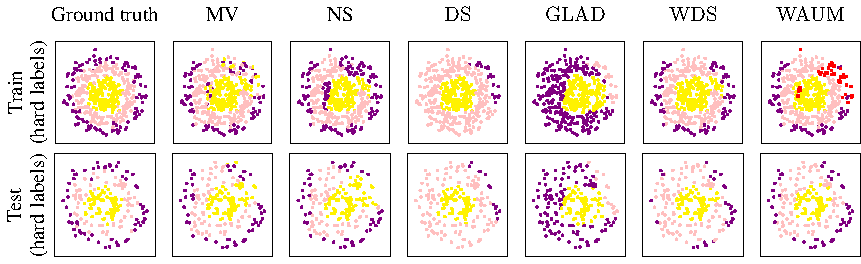
\includegraphics[width=.8\textwidth]{images/Preds3circles}
    \caption{\texttt{three\_circles}: One realization of \Cref{tab:res3circles} varying the aggregation strategy. Training labels are provided from \Cref{fig:threecircles_workers} and predictions on the test set are from three dense layers' artificial neural network $(30, 20, 20)$ trained on the aggregated soft labels. For ease of visualization, the color displayed for each task represents the most likely class.
        Red points are pruned from training by $\mathrm{WAUM}$ with threshold $\alpha=0.1$. Here, we have $n_{\texttt{task}}=525$.
        $\mathrm{WAUM}$ method as in \Cref{tab:res3circles} uses $\mathrm{WDS}$ labels.
        }
    \label{fig:threecircles_predictions}
\end{figure}

We simulate three cloud points (to represent $K=3$ classes) using \texttt{scikit-learn}'s function \texttt{two\_circles}; see \Cref{fig:threecircles_workers}.
The $n_\texttt{worker}=3$ workers are standard classifiers: $w_1$ is a linear Support Vector Machine Classifier (linear SVC), $w_2$ is an SVM with RBF kernel (SVC), and $w_3$ is a gradient boosted classifier (GBM).
Data is split between train (70\%) and test (30\%) for a total of $750$ points and each simulated worker votes for all tasks, \emph{i.e.} for all $x\in\mathcal{X}_\texttt{train}$, $|\mathcal{A}(x)|=n_\texttt{worker}=3$, leading to $n_{\texttt{task}}=525$ tasks (points).
The performance reported in \Cref{tab:res3circles} is averaged over $10$ repetitions.

\begin{figure}[tbh]
    \centering
    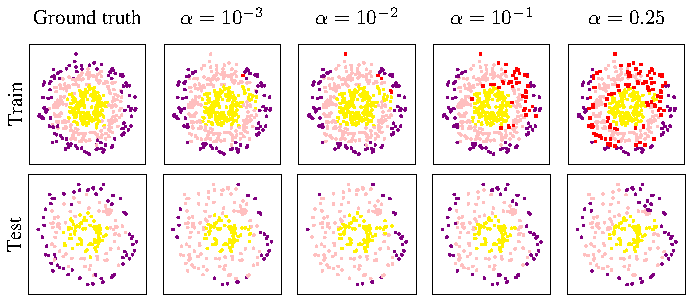
\includegraphics[width=.75\linewidth]{images/Simu3circlesAlpha.pdf}
    \caption{Influence of $\alpha$ on the pruning step. Red dots indicate data points pruned from the training set, at level $q_\alpha$ in the $\mathrm{WAUM}$ (see line 10 in \Cref{alg:WAUMstack}).
        We consider ($\alpha\in\{10^{-3}, 10^{-2}, 10^{-1}, 0.25\}$).
        The neural network used for predictions is three dense layers
        $(30, 20, 20)$, as for other simulated experiments.
        Training labels are from the $\mathrm{WDS+WAUM}$ strategy with performance reported in \Cref{tab:res3circles}.
        The more we prune data, the worse the neural network can learn from the training dataset.
        However, removing the tasks with high disagreement noise helps to generalize.
        }    \label{fig:three_circles_alpha_influence}
\end{figure}

\begin{figure}[thb]
    \centering
    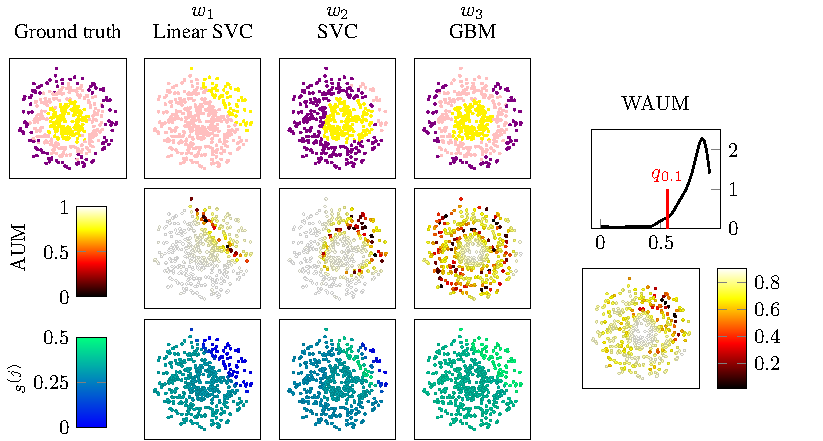
\includegraphics[width=.75\linewidth]{images/Simu3circles}
    \caption{$\texttt{three\_circles}$: one realization of simulated workers $w_1,w_2,w_3$, with their $\mathrm{AUM}$, normalized trust scores $s^{(j)}$ (left) and $\mathrm{WAUM}$ distributions (right) for $\alpha=0.1$. Worker $w_1$ has less impact on the final $\mathrm{WAUM}$ in the disagreement area. Note also that for worker $w_1$ (LinearSVC), the region with low $\mathrm{AUM}$ values recovers the usual classifier's margin around the decision boundary.}
    \label{fig:threecircles_workers}
\end{figure}

\begin{table}[tbh]
    \centering
        \begin{tabular}{m{4.9cm}cc}
            Strategy              & $\mathrm{Acc}_{\texttt{test}}$ & ECE                      \\ \hline \\[-0.2cm]
            $\mathrm{MV}$                   & $0.73\pm 0.03$                 & $\mathbf{0.13}\pm 0.03$                         \\
            $\mathrm{NS}$                   & $0.70\pm 0.02$                 & $0.18\pm 0.02$                                  \\
            $\mathrm{DS}$                   & $0.75\pm 0.07$                 & $0.22\pm 0.08$                                \\
            $\mathrm{GLAD}$                 & $0.58\pm 0.02$                 & $0.36\pm 0.02$                             \\
              \rowcolor{gray!20}$\mathrm{WDS}$                  & $0.81\pm 0.04$                 & $0.17\pm 0.03$                                \\
                 \rowcolor{gray!20}$\mathrm{WDS+AUMC}(\alpha=10^{-1})$                  & $0.81\pm 0.02$                 & $0.17\pm 0.01$                                \\
              \rowcolor{gray!20}$\mathrm{WDS+WAUM}(\alpha=10^{-2})$ & $0.80\pm 0.04$                 & $0.17\pm 0.01$\\
              \rowcolor{gray!20}$\mathrm{WDS+WAUM}(\alpha=10^{-1})$ & $\mathbf{0.83}\pm 0.03$        & $0.19\pm 0.04$                             \\
              \rowcolor{gray!20}$\mathrm{WDS+WAUM}(\alpha=0.25)$    & $0.69\pm 0.02$                 & $0.19\pm 0.02$
            \end{tabular}
        \caption{\texttt{three\_circles}: Aggregation and learning performance presented in \Cref{fig:threecircles_predictions} ($n_\texttt{task}=525$ tasks, $|\mathcal{A}(x)|=n_\texttt{worker}=3$, $10$ repetitions). Errors represented are standard deviations.
        Note that the best worker, $w_3$, reaches
        % $0.92$ training accuracy and
        $0.84$ on test accuracy.
        }
        \label{tab:res3circles}
\end{table}

A disagreement area is identified in the northeast area of the dataset (see \Cref{fig:threecircles_workers}).
\Cref{tab:res3circles} also shows that pruning too little data ($\alpha$ small) or too much ($\alpha$ large) can mitigate the performance.
In \Cref{fig:three_circles_alpha_influence}, we show the impact of the pruning hyperparameter $\alpha$. The closer $\alpha$ is to $1$, the more training tasks are pruned from the training set (and the worse the performance).

\subsubsection*{Two moons simulation}

This dataset is introduced as a case where pruning is not recommended, to illustrate the limitations of the $\textrm{worker-wise WAUM}$ method.
The \texttt{two\_moons} simulation framework showcases the difference between relevant ambiguity in a dataset and an artificial one.
This dataset is created using \texttt{make\_moons} function from \texttt{scikit-learn}.
We simulate $n_\texttt{task}=500$ points, a noise $\varepsilon=0.2$ and use a test split of $0.3$.

\begin{figure}[thb]
    \centering
    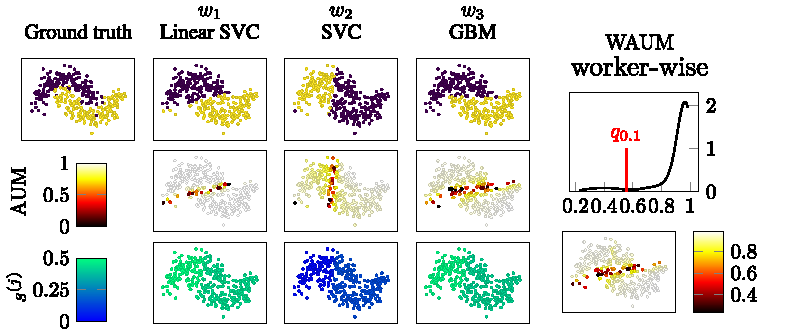
\includegraphics[width=0.75\textwidth]{images/SimuMoons}
    \caption{$\texttt{two\_moons}$ dataset: simulated workers with associated $\mathrm{AUM}$ and normalized trust scores. The hyperparameter $\alpha$ is set to $0.1$ for the $\textrm{worker-wise WAUM}$.
        Notice that the $\mathrm{SVC}$ classifier is mostly wrong (since we only train for one epoch for this worker), inducing a lower trust score overall.}
    \label{fig:2moons_workers}
\end{figure}

\begin{figure}[thb]
    \centering
    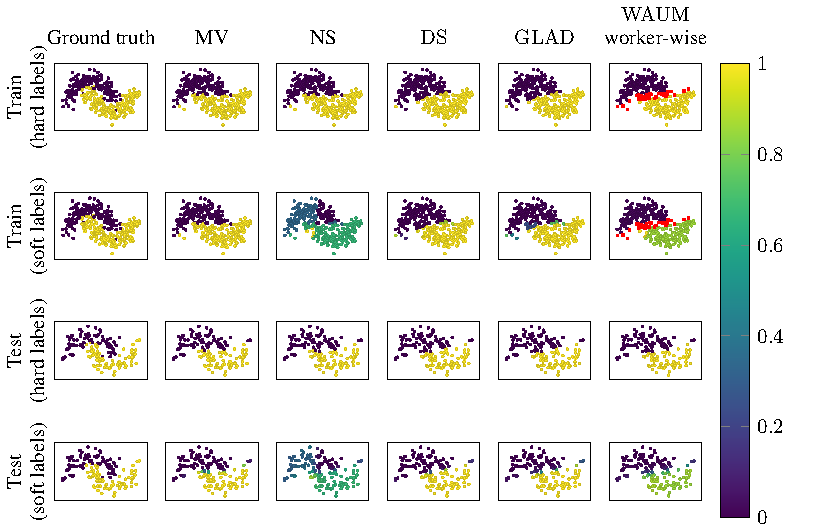
\includegraphics[width=0.75\textwidth]{images/PredsMoons}
    \caption{ \texttt{two\_moons} dataset: One realization of \Cref{tab:results_simu_moons} varying the aggregation strategy. Label predictions on train/test sets provided by a three dense layers' artificial neural network $(30, 20, 20)$ trained on smooth labeled obtained after aggregating the crowdsourced labels (as in \Cref{fig:2moons_workers}).
        Points in red are pruned from the training set in the $\textrm{worker-wise WAUM}$ aggregation.
        The $\alpha$ hyperparameter is set to $0.1$. Each point represents a task $x_i$, and its color is the probability of belonging in class $1$.
        One can visualize the ambiguity in the soft training aggregated labels, but also in the resulting predictions by the neural network. Errors represented are standard deviations.}
    \label{fig:twomoons_predictions_soft}
\end{figure}

\begin{table}[H]
    \centering
    \caption{Training and test accuracy depending on the aggregation method used for the \texttt{two\_moons}'s dataset with $n_\texttt{task}=500$ points used for training a three dense layers' artificial neural network $(30, 20, 20)$. For reference, the best worker is $w_3$ with a training accuracy of $0.923$ and a test accuracy of $0.900$. }
        \begin{tabular}{lccc}
            Aggregation                                  & $\mathrm{Acc}_{\text{test}}$ & ECE
            \\ \hline \\
            MV                                                           & $\mathbf{0.894\pm 0.002}$    & $\mathbf{0.098}\pm 0.004$ \\
            NS                                                             & $0.887\pm 0.002$    & $0.217\pm 0.010$          \\
            DS                                                         & $0.867\pm 0.000$             & $0.126\pm 0.001$          \\
            $\mathrm{GLAD}$                                                  & $0.872\pm 0.006$             & $0.107\pm 0.004$          \\
             \rowcolor{gray!20}$\mathrm{WDS}+\mathrm{WAUM}(\alpha=10^{-3}) $                     & $0.875\pm 0.002$             & $0.088\pm 0.012$ \\
             \rowcolor{gray!20}$\mathrm{WDS}+\mathrm{WAUM}(\alpha=10^{-2})$                  & $0.874\pm 0.002$             & $0.092\pm 0.011$ \\
             \rowcolor{gray!20}$\mathrm{WDS}+\mathrm{WAUM}(\alpha=10^{-1})$                    & $0.870\pm 0.003$             & $0.101\pm 0.020$          \\
             \rowcolor{gray!20}$\mathrm{WDS}+\mathrm{WAUM}(\alpha=0.25)$                     & $0.829\pm 0.006$             & $0.135\pm 0.011$          \\
        \end{tabular}
    \label{tab:results_simu_moons}
\end{table}
As can be observed with \Cref{fig:2moons_workers} and \Cref{fig:twomoons_predictions_soft}, the difficulty of this dataset comes from the two shapes leaning into one another.
However, this intrinsic difficulty is not due to noise but is inherent to the data.
In this case, removing the hardest tasks means removing points at the edges of the crescents, and those are important in the data's structure.
From \Cref{tab:results_simu_moons}, we observe that learning on naive soft labeling leads to better performance than other aggregations.
But with these workers, no aggregation produced labels capturing the shape of the data.

\subsection{Results on real datasets}
In this section, we investigate three popular crowdsourced datasets: \texttt{CIFAR-10H}, \texttt{LabelMe} and \texttt{Music}.
The first one, \texttt{CIFAR-10H} \citep{peterson_human_2019}, is a curated dataset with many votes per task while \texttt{LabelMe} \citep{rodrigues2018deep} and \texttt{Music} \citep{rodrigues2014gaussian} datasets are more challenging, having fewer labels per task.
This low number of votes per task, especially for $\texttt{LabelMe}$ can lead to erroneous MV labels which then impact the quality of the $\mathrm{AUMC}$. In this context, the label distribution's entropy is also a poor choice to identify hard tasks as can be seen in \Cref{fig:entropy_vs_waum}.
Indeed, with up to three labels, the entropy can only take four different values and thus is no help in ranking the difficulty of $1000$ tasks.

To prune only a few tasks, we choose $\alpha = 1\%$ for \texttt{CIFAR-10H} and \texttt{LabelMe} datasets.
For the \texttt{Music} dataset, $\alpha=5\%$ leads to better generalization performance; considering the dataset size and complexity, picking $\alpha=0.1$ would lead to worse performance.
Ablation studies by architecture are performed on \texttt{CIFAR-10H} and \texttt{LabelMe} datasets in \Cref{fig:tab_arch} to show consistent improvement in performance by using the $\mathrm{WAUM}$ to prune ambiguous data.

\begin{figure}[tbh]
    \centering
    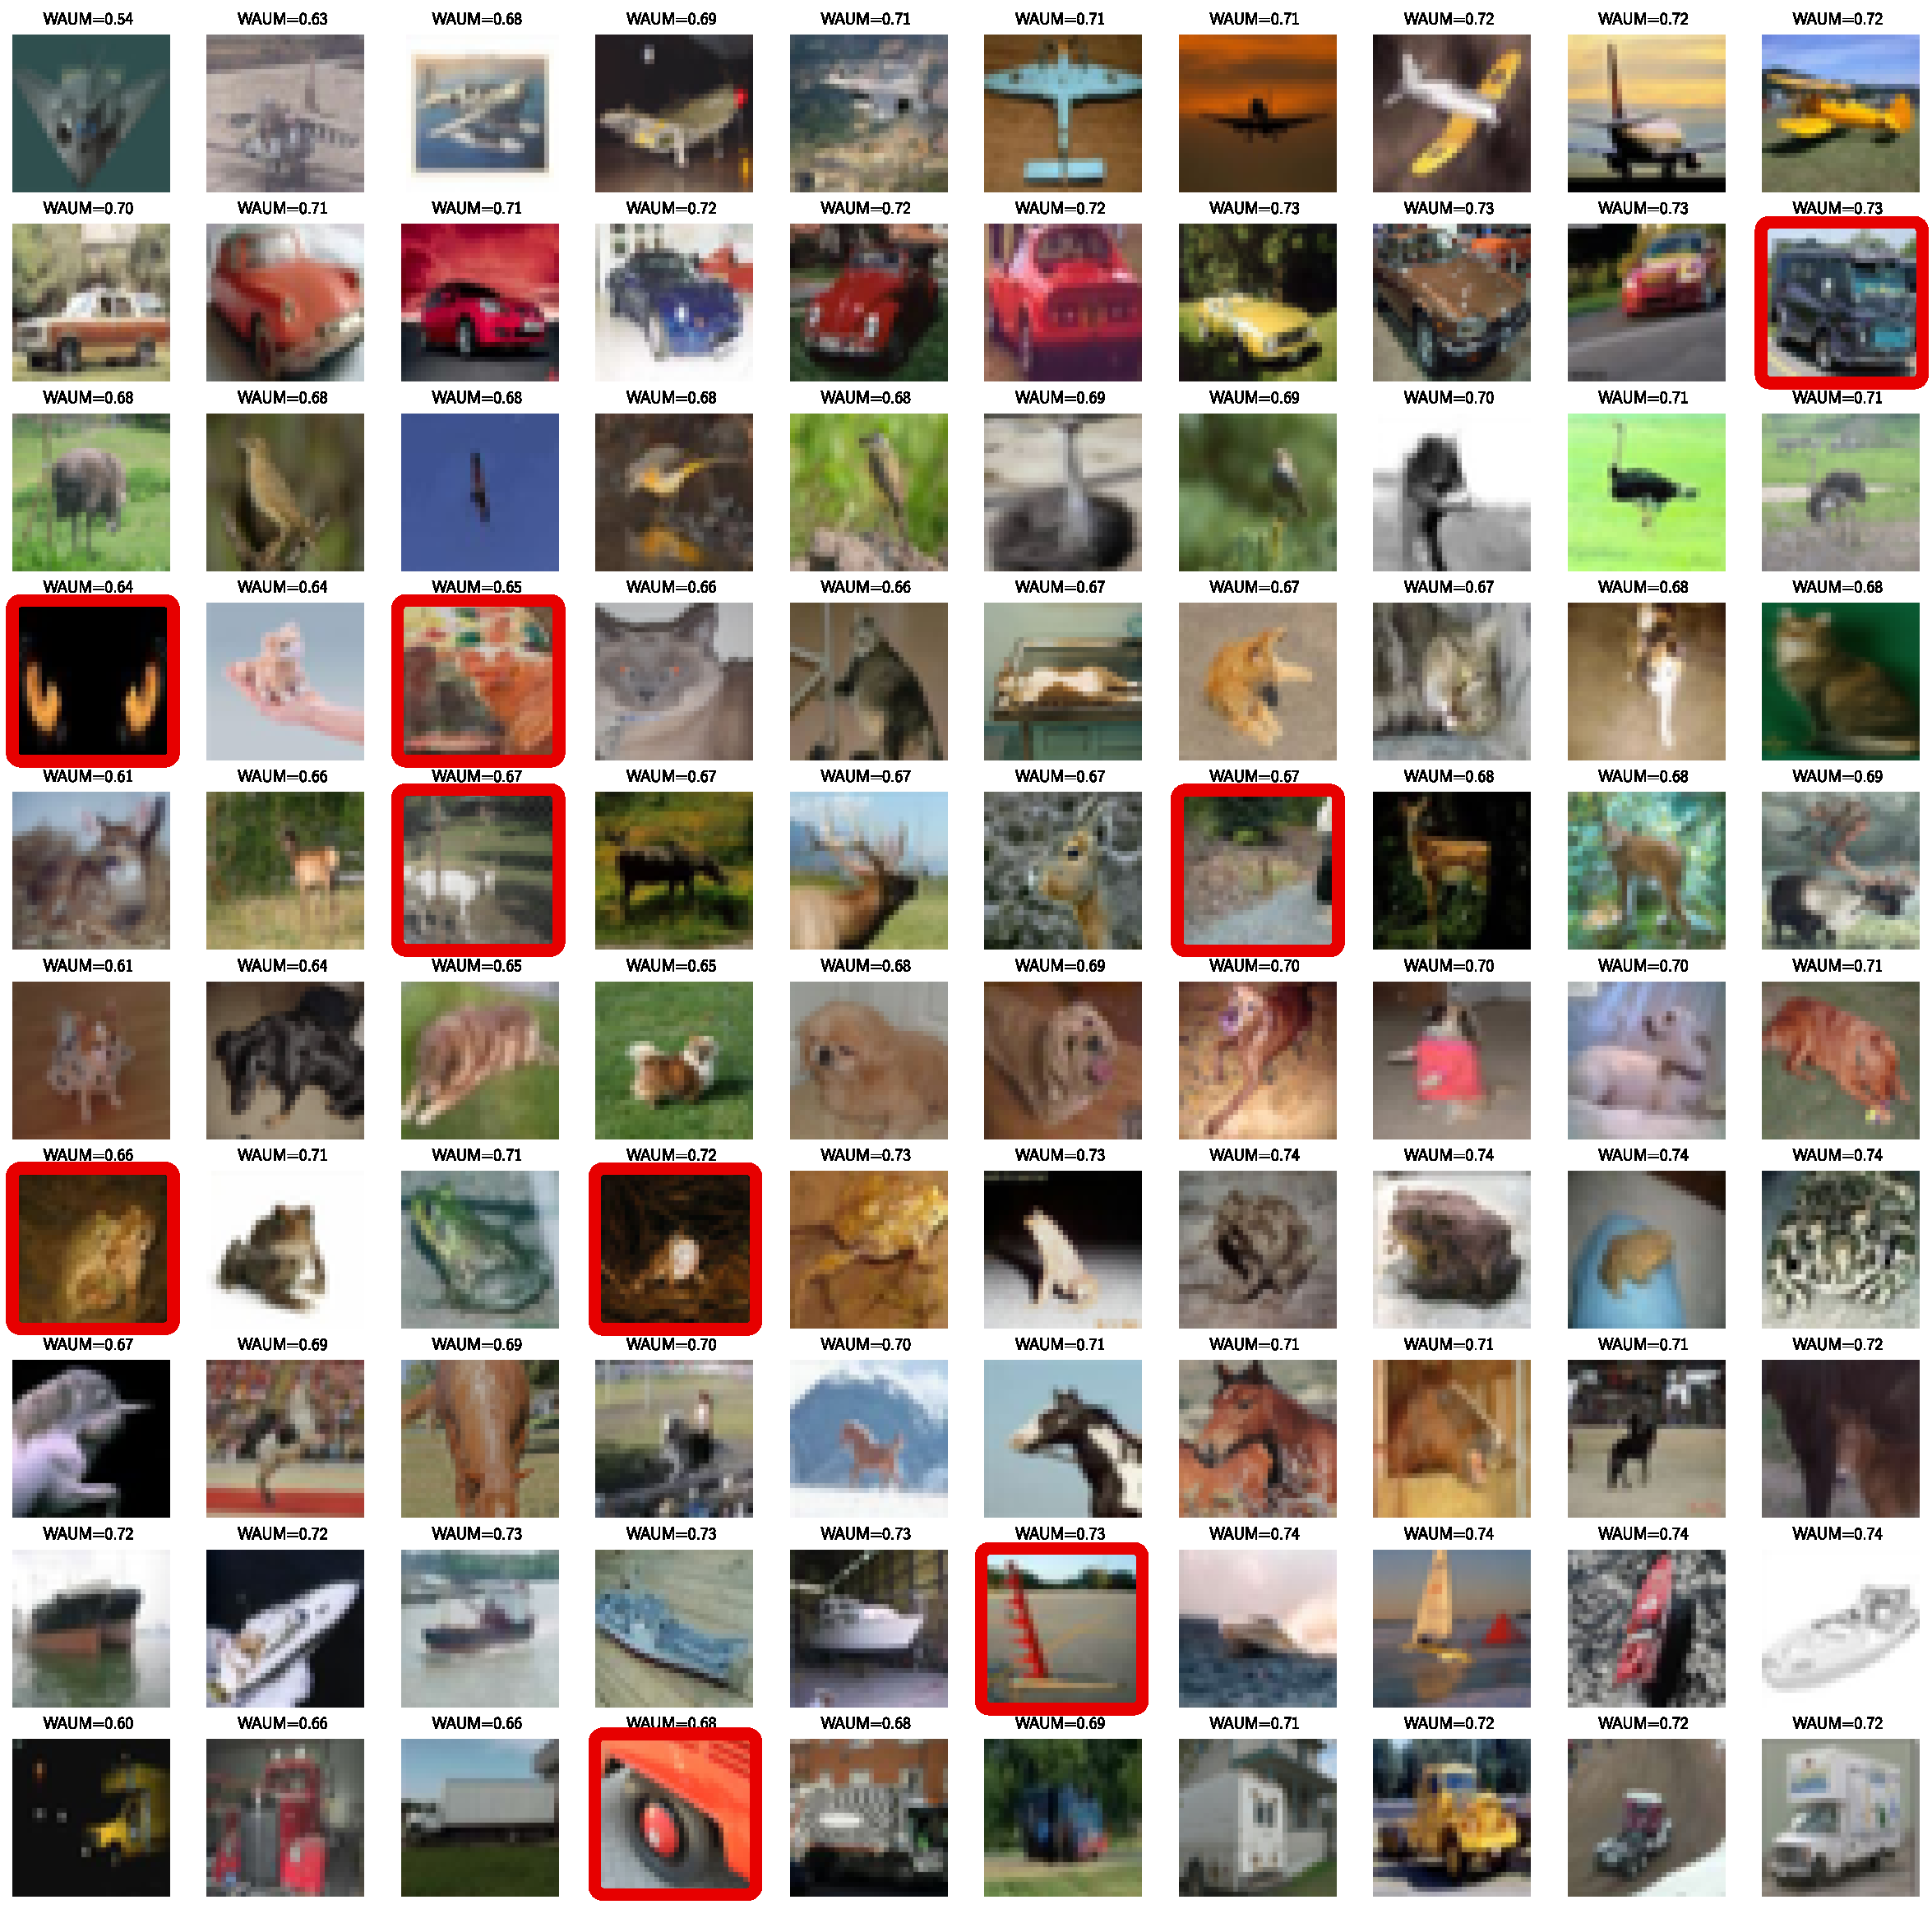
\includegraphics[width=0.9\columnwidth]{images/lowest_waum_C10H_yang_Yang_True_red.pdf}
    \caption{\texttt{CIFAR-10H}: 10 worst images for $\mathrm{WAUM}$ scores, by labels given in CIFAR-10. The rows represent the labels \texttt{airplane}, \texttt{automobile}, \texttt{bird}, \texttt{cat}, \texttt{deer}, \texttt{dog}, \texttt{frog}, \texttt{horse}, \texttt{ship}, and \texttt{truck}. Images in red can be particularly hard to classify as they are not typical examples of their label. Comparison with the $\mathrm{AUMC}$ and the $\mathrm{AUM}$ are available in \Cref{fig:comparison_waums_aumc} \Cref{subsubsec:cifar-10h_dataset}.}
    \label{fig:worse_C10H}
\end{figure}

\subsubsection*{\texttt{CIFAR-10H} dataset.} The training part of \texttt{CIFAR-10H} consists of the $10\,000$ tasks extracted from the test set of the classical CIFAR-10 dataset \citep{krizhevsky2009learning}, and $K=10$.
A total of $n_\texttt{worker}=2571$ workers participated on the Amazon Mechanical Turk platform, each labeling $200$ images ($20$ from each original class), leading to approximately $50$ answers per task.
We have randomly extracted $500$ tasks for a validation set (hence $n_{\texttt{train}}=9500$).
This dataset is notoriously more curated \citep{aitchison2020statistical} than a common dataset in the field: most difficult tasks were identified and removed at the creation of the CIFAR-10 dataset, resulting in few ambiguities.
\Cref{tab:spam-0-expe} shows that in this simple setting, our data pruning strategy is still relevant, with the choice $\alpha=0.01$. Images with worst $\mathrm{WAUM}$ for each class are presented in \Cref{fig:worse_C10H}.

Furthermore, the $\mathrm{WAUM}$ leads to better generalization performance than the vanilla DS model and the pruning with $\mathrm{AUMC}$.
Overall, we show that there is a gain in performance obtained by using a pruning preprocessing step compared to training the classifier on the aggregated labels for the full training set.
There is consistently an improvement in using the $\mathrm{WAUM}$ pruning -- which weights the margins by worker and tasks -- over the naive $\mathrm{AUMC}$ which does not use reweighing.


\texttt{CIFAR-10H} is a relatively well-curated dataset, and we observe in \Cref{tab:spam-0-expe} that in this case, simple aggregation methods already perform well, in particular NS.
Over the $2571$ workers, less than $20$ are identified as spammers using \citet{raykar_ranking_2011} but note that most difficult tasks were removed when creating the original CIFAR-10 dataset.
We refer to the \emph{"labeler instruction sheet"} of \citet[Appendix C]{krizhevsky2009learning} for more information about the directives given to workers.

\begin{table}[t]
    \label{tab:spam-0-expe}
    \begin{footnotesize}
        \begin{center}
            \begin{tabular}{lcc}
                Strategy & $\mathrm{Acc}_{\texttt{test}} (\%)$ & $1-\mathrm{ECE}$
                \\ \hline \\[-0.2cm]
                MV                 & $69.53\pm 0.84$               & $0.825\pm 0.00$                                 \\
                MV + AUMC & $71.12\pm 1.12$ & $\mathbf{0.836\pm 0.01}$ \\
                MV + WAUM & $\mathbf{72.34\pm 1.01}$ & $0.814\pm 0.02$ \\
                \rowcolor{gray!20}NS                 & $72.14\pm 2.74$               & $\mathbf{0.868\pm 0.03}$          \\
                \rowcolor{gray!20}NS + AUMC                 & $71.80\pm 2.12$               & $0.838\pm 0.00$          \\
                \rowcolor{gray!20}NS + WAUM                 & $\mathbf{72.21\pm 1.82}$               & $0.829\pm 0.00$          \\
                DS                 & $70.26\pm 0.93$               & $0.827\pm 0.00$             \\
                DS + AUMC                 & $70.43\pm 1.10$               & $\mathbf{0.833\pm 0.02}$             \\
                DS + WAUM                & $\mathbf{72.71\pm 0.98}$               & $0.814\pm 0.02$             \\
               \rowcolor{gray!20} $\mathrm{GLAD}$    & $70.28\pm 0.88$               & $\mathbf{0.838\pm 0.01}$\\
                \rowcolor{gray!20} $\mathrm{GLAD}$ + AUMC    & $70.42\pm 1.23$               & $0.830\pm 0.01$\\
               \rowcolor{gray!20} $\mathrm{GLAD}$ + WAUM    & $\mathbf{71.93\pm 1.12}$               & $0.812\pm 0.02$\\
                  WDS                & $72.49\pm 0.48$               & $\mathbf{0.868\pm 0.00}$         \\
                  WDS + AUMC                & $72.47\pm 0.45$               & $0.866\pm 0.00$         \\

                  $\mathrm{WDS} + \mathrm{WAUM}$    & $\mathbf{72.67\pm 0.59}$      & $\mathbf{0.868 \pm 0.00}$
            \end{tabular}
        \end{center}
    \end{footnotesize}
    \caption{\texttt{CIFAR-10H}: performance of a \texttt{ResNet-18} by label-aggregation crowdsourcing strategy ($\alpha=0.01$). Errors represented are standard deviations.}
\end{table}


% Source: tanguy_phd/reproducible_paper/labelme/extract_results.py
\begin{figure}[htb]
    \label{fig:labelme_worstWAUM}%
    \centering
    \hfill
    \subfloat[Label \texttt{street}.]{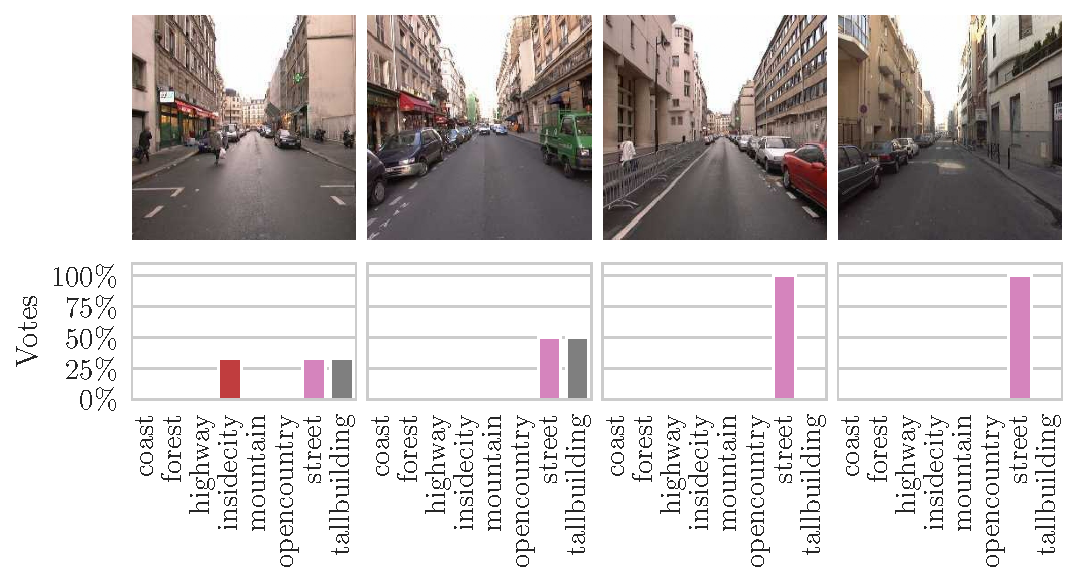
\includegraphics[width=0.49583\textwidth]{images/street_and_distrib}}
    \hfill
    \subfloat[Label \texttt{tallbuilding}.]{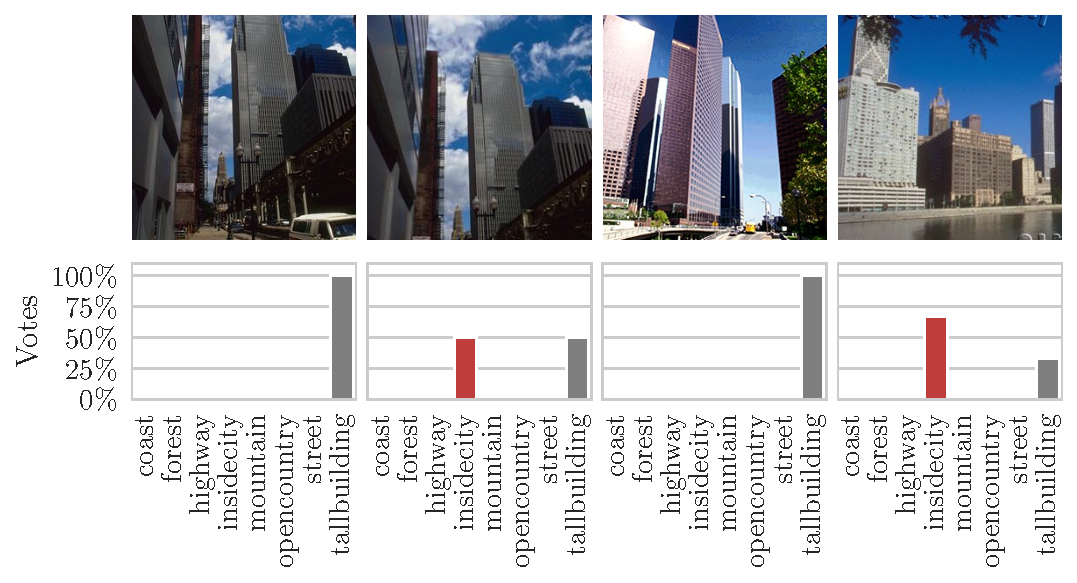
\includegraphics[width=0.49583\textwidth]{images/tallbuilding_and_distrib}}
    \caption{\texttt{LabelMe} dataset: Worst $\mathrm{WAUM}$ for classes (top) and the associated voting distribution for each image (bottom). (a) Label \texttt{street} (b)  Label \texttt{tallbuilding}.
        Even if the two tasks are very similar, because the workers are different the associated proposed labels can differ and add noise during training.}
\end{figure}

\begin{figure}[th]
    \centering
    \begin{minipage}{0.45\textwidth}
        \centering
        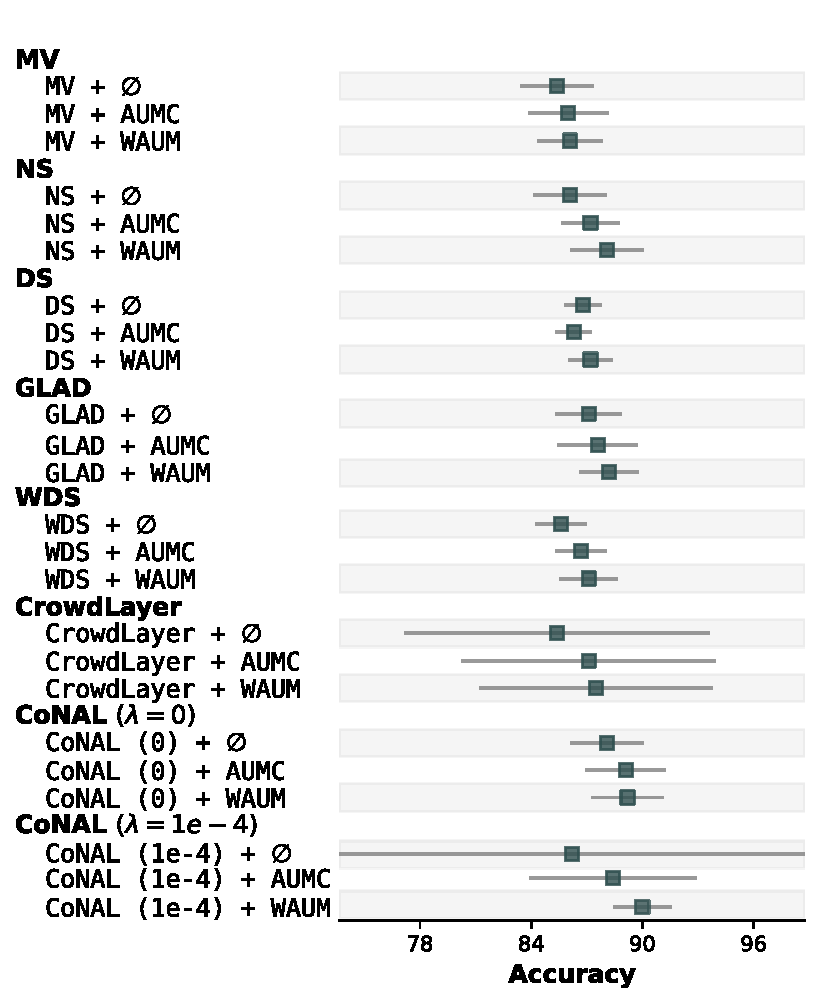
\includegraphics[width=\linewidth]{images/Accuracy_foresplot_labelme.pdf}
        \label{fig:forest_labelme_accuracy}
    \end{minipage}
    \hfill
    \begin{minipage}{0.45\textwidth}
        \centering
        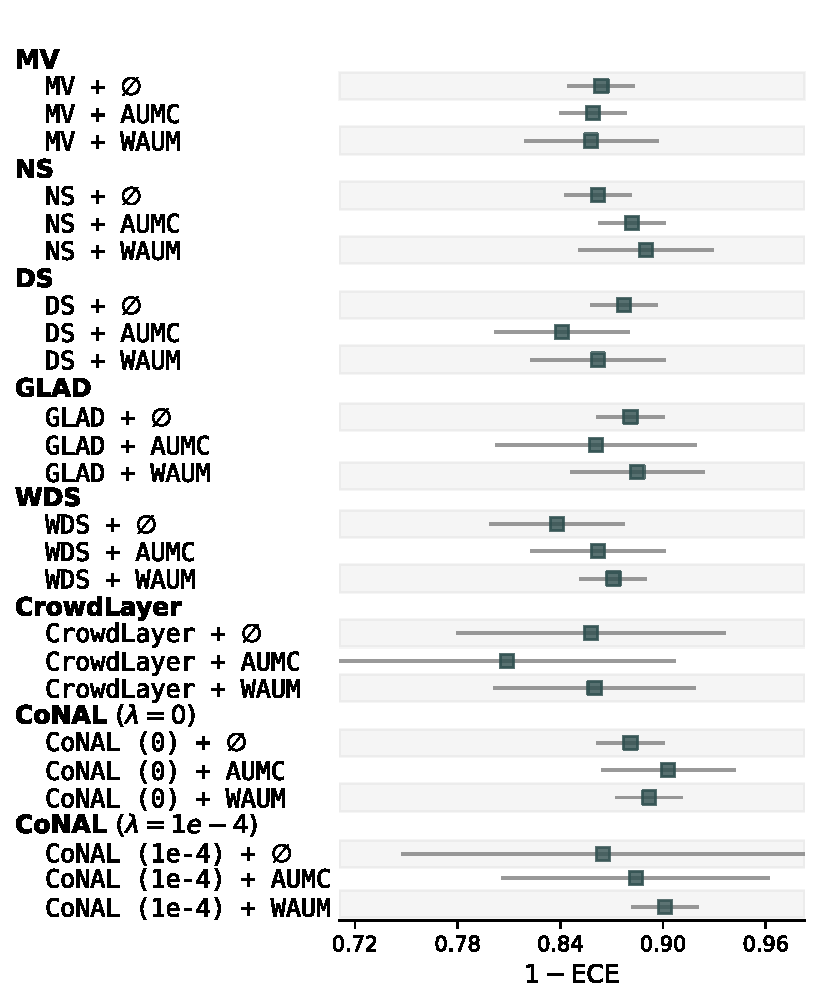
\includegraphics[width=\linewidth]{images/ECE_foresplot_labelme.pdf}
        \label{fig:forest_labelme_ece}
    \end{minipage}
    \caption{Ablation study on \texttt{LabelMe} using the VGG backbone: $\alpha=0.01$. Errors are Gaussian confidence intervals at $95\%$.}
    \label{fig:forest_labelme}
\end{figure}

\subsubsection{\texttt{LabelMe} dataset.} This dataset consists in classifying $1000$ images in $K=8$ categories.
In total $77$ workers are reported in the dataset (though only $59$ of them answered any task at all).
Each task has between $1$ and $3$ labels. A validation set of $500$ images and a test set of $1188$ images are available.

We observe in \Cref{fig:forest_labelme} that the $\mathrm{WAUM}$ improves the final test accuracy when combined with the CoNAL network with regularization.
Note that the \texttt{LabelMe} dataset has classes that overlap and thus lead to intrinsic ambiguities.
This is the reason why the CoNAL strategy was introduced by \citet{chu2021learning}: modeling common confusions helps the network's decision, so it was expected for the CoNAL to perform well.
Combined with our $\mathrm{WAUM}$, additional gains are obtained on both metrics.
The vanilla strategy, either for aggregation or learning, can be improved using a pruning preprocessing step.
However, between the $\mathrm{AUMC}$ and the $\mathrm{WAUM}$, we show a consistent improvement in using the $\mathrm{WAUM}$ that considers weights for the workers individually.
For example, the classes \texttt{highway}, \texttt{insidecity}, \texttt{street} and \texttt{tallbuilding} (in rows) are overlapping for some tasks: cities have streets with tall buildings, leading to confusion shown in \Cref{fig:worse_labelme}.

\begin{figure}[t]
    \centering
    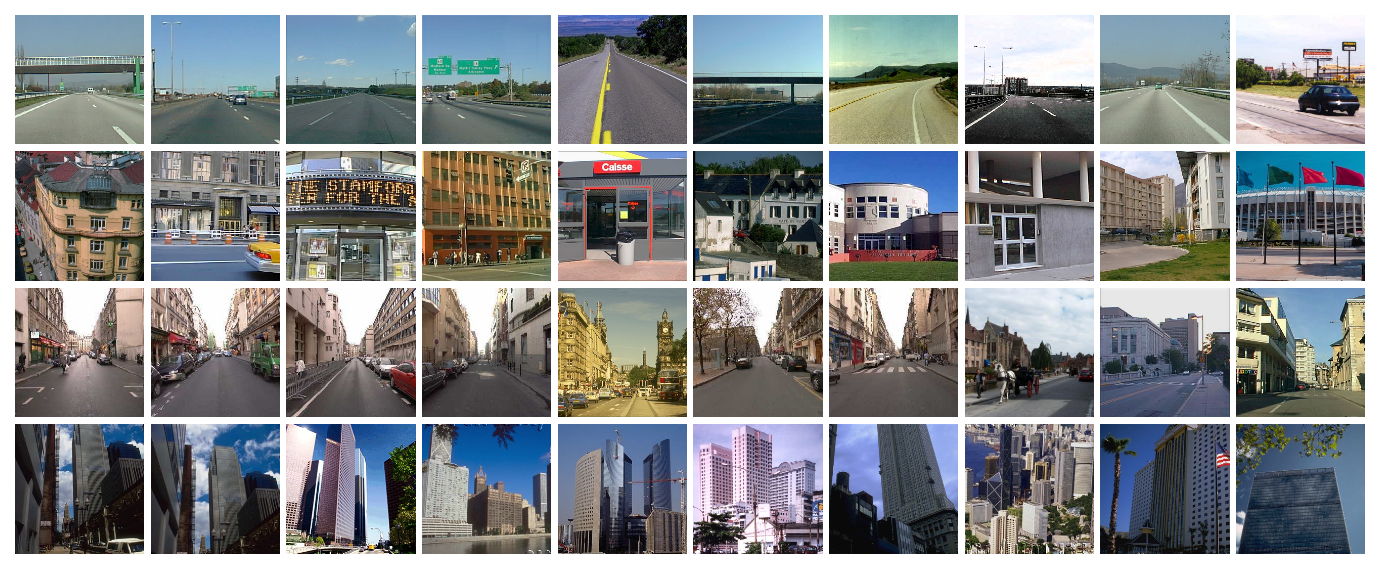
\includegraphics[width=0.9\columnwidth]{images/lowest_labelme_highway_insidecity_street_tallbuilding.pdf}
    \caption{\texttt{LabelMe}: top-$10$ worst images  detected by the $\mathrm{WAUM}$ (with labels row-ordered from top to bottom: \texttt{highway}, \texttt{insidecity}, \texttt{street}, \texttt{tallbuilding}). Overlapping classes lead to labeling confusion and learning difficulties for both the workers and the neural network.}
    \label{fig:worse_labelme}
\end{figure}

\subsubsection*{\texttt{Music} dataset.}

\begin{figure}[thb]
    \centering
    \begin{minipage}{0.45\textwidth}
        \centering
        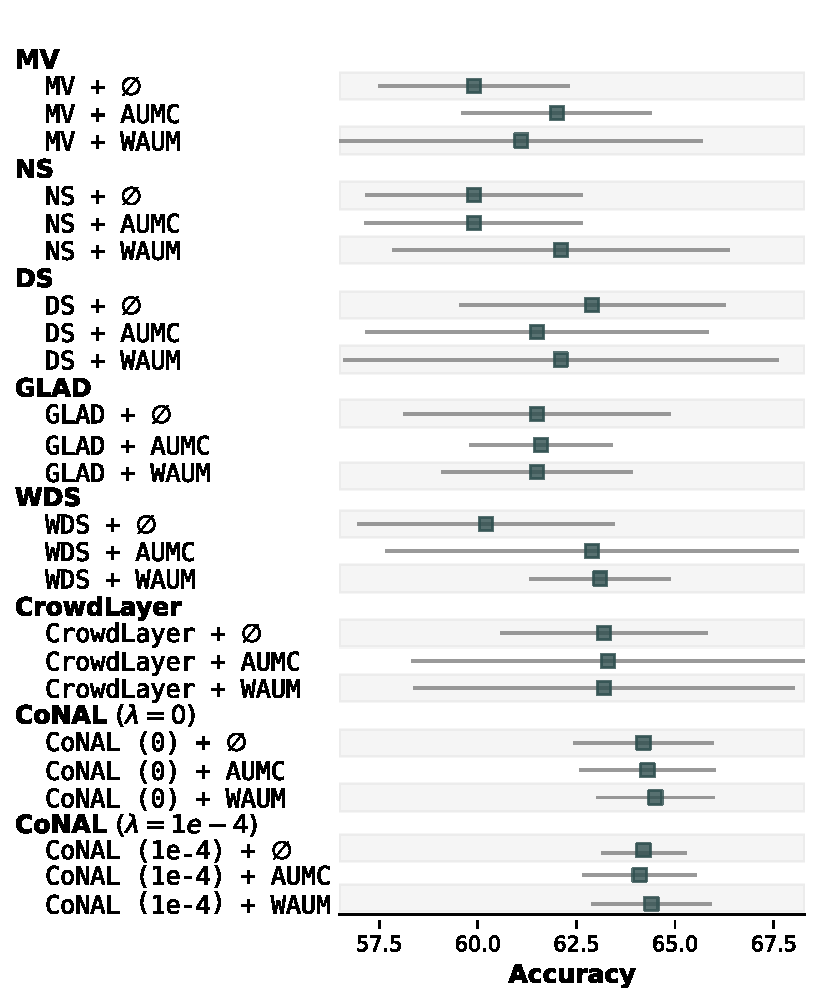
\includegraphics[width=\linewidth]{images/Accuracy_foresplot_music.pdf}
        \label{fig:forest_music_accuracy}
    \end{minipage}
    \hfill
    \begin{minipage}{0.45\textwidth}
        \centering
        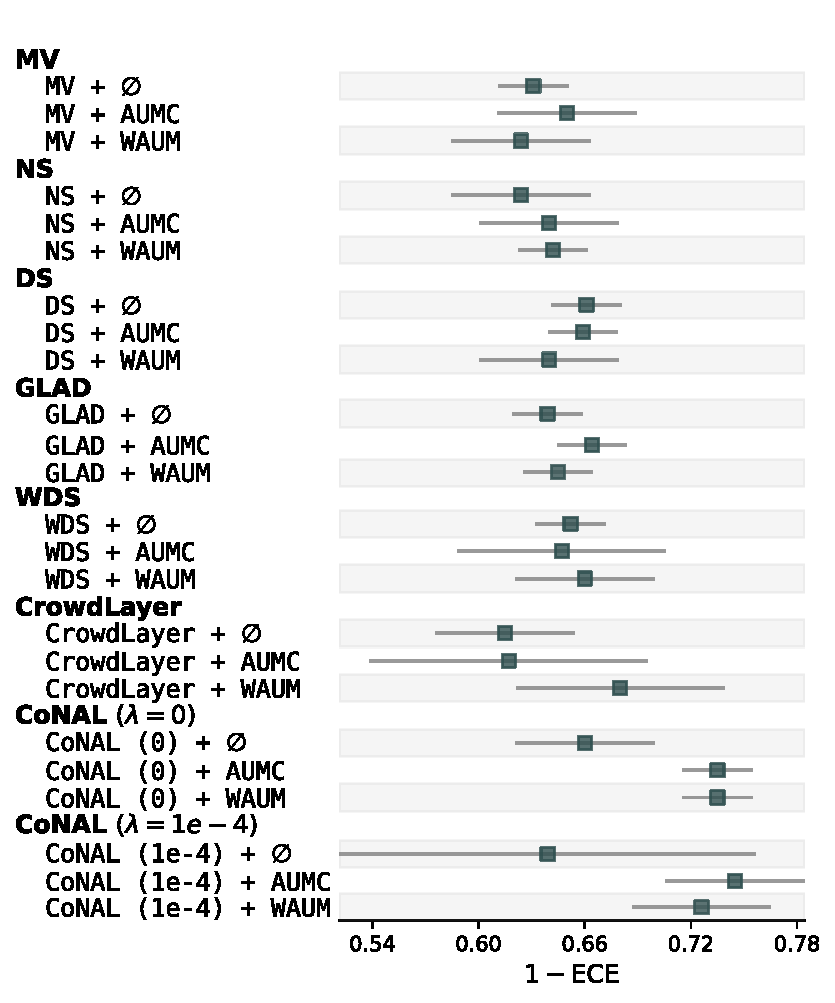
\includegraphics[width=\linewidth]{images/ECE_foresplot_music.pdf}
        \label{fig:forest_music_ece}
    \end{minipage}
    \caption{Ablation study on \texttt{Music} using the VGG backbone: $\alpha=0.05$. Errors are Gaussian confidence intervals at $95\%$.}
    \label{fig:forest_music}
\end{figure}

This dataset differs from \texttt{LabelMe} and \texttt{CIFAR-10H} as it consists in classifying $1000$ recordings of $30$ seconds into $K=10$ music genres.
All the $44$ workers involved voted for at least one music, resulting in up to $7$ labels per task.
Instead of classifying the original audio files, we use the associated Mel spectrograms following the methodology considered by \citet{dong2018convolutional} to retrieve an image classification setting.
Though the benefits are not as striking as before on test accuracy, the ECE is slightly improved by combining our $\mathrm{WAUM}$ with $\mathrm{CoNAL}$ as can be seen in \Cref{fig:forest_music}.
Moreover, we show constant improvement of the test generalization performance using the $\mathrm{WAUM}$ preprocessing either in accuracy or in calibration.

Among other interesting discoveries, the $\texttt{WAUM}$ helped us detect that the music \emph{Zydeco Honky Tonk} by Buckwheat Zydeco was labeled as \texttt{classical}, \texttt{country} or \texttt{pop} by the workers, though it is a \texttt{blues} standard.
Another example is \emph{Caught in the middle} by Dio classified (with the same number of votes) as \texttt{rock}, \texttt{jazz}, or \texttt{country} though it is a \texttt{metal} song.
One last example detected: the music \emph{Patches} by Clarence Carter is stored in the \texttt{disco00020.wav} file.
The true label is supposed to be \texttt{disco}, while the workers have provided the following labels: two have chosen \texttt{rock}, two \texttt{blues}, one \texttt{pop} and another one proposed \texttt{country}.
The actual genre of this music is \texttt{country}-soul, so both the true label and five out of six workers are incorrect.

\subsubsection*{WAUM sensitivity to the neural network architecture.}
\begin{figure}[th]
  \centering
  \begin{tabular}{m{1.75cm} *{4}{>{\centering\arraybackslash}m{.15\linewidth}}}
    \centering CIFAR-10H & \multicolumn{2}{c}{\raisebox{-.5\height}{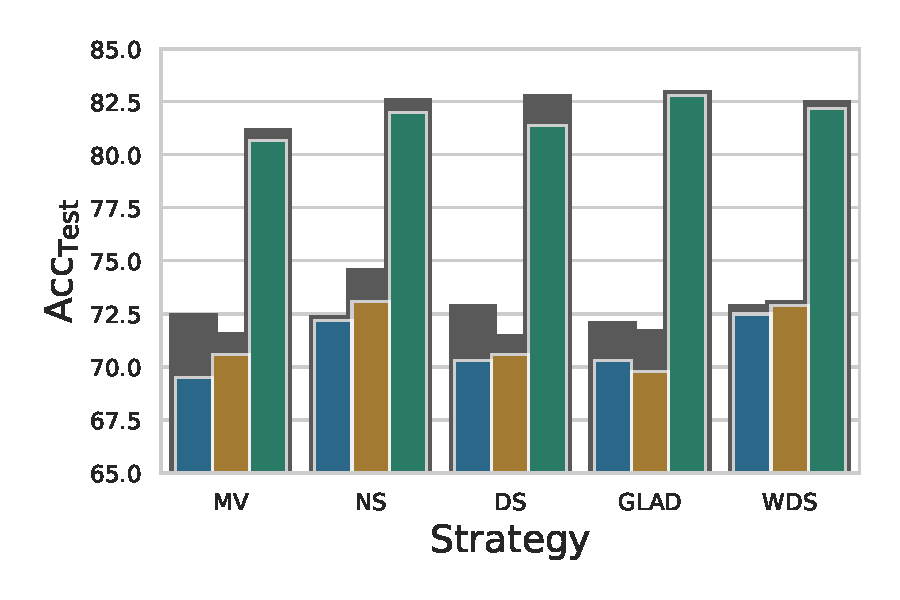
\includegraphics[width=0.4\linewidth]{images/acc_cifar10H.pdf}}} &
    \multicolumn{2}{c}{\raisebox{-.5\height}{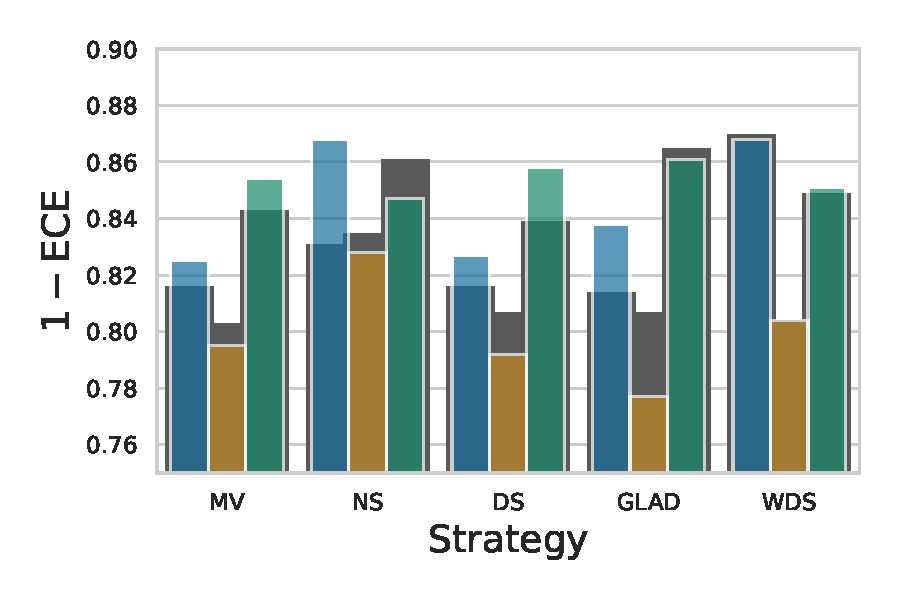
\includegraphics[width=0.4\linewidth]{images/ECE_cifar10H.pdf}} }\\
    \centering LabelMe & \multicolumn{2}{c}{\raisebox{-.5\height}{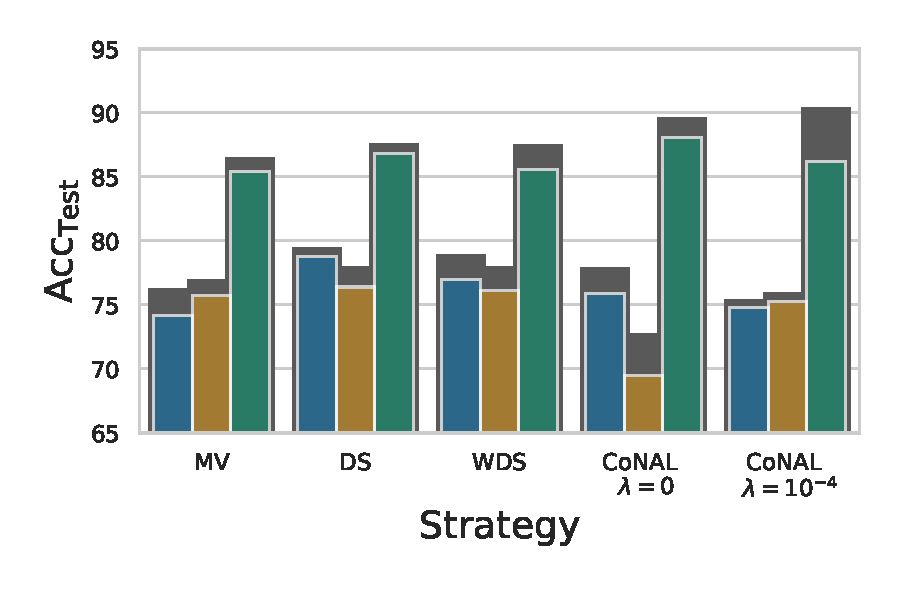
\includegraphics[width=0.4\linewidth]{images/acc_labelme.pdf} }}&
    \multicolumn{2}{c}{\raisebox{-.5\height}{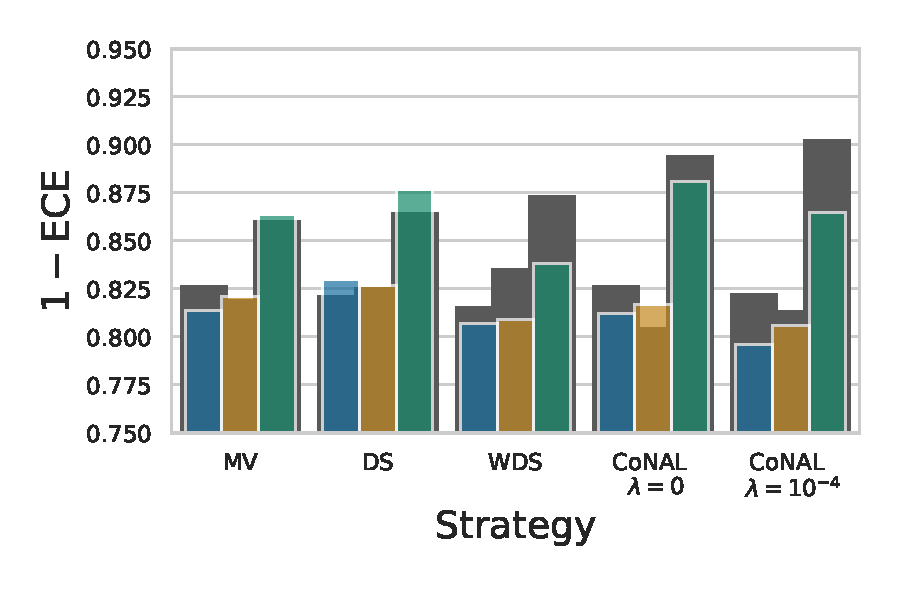
\includegraphics[width=0.4\linewidth]{images/ECE_labelme.pdf}}} \\
    &\multicolumn{4}{c}{
\includegraphics[width=0.75\linewidth]{images/legend_ablation_study.pdf}} \\
  \end{tabular}
  \caption{Performance obtained by training on the pruned dataset from the $\mathrm{WAUM}$ preprocessing step on \texttt{CIFAR-10H} and \texttt{LabelMe}. We consider multiple neural network architectures -- ResNet-18, ResNet-34 or VGG-16 with batch normalization and two supplementary dense layers. We show that performance in accuracy is improved in most cases. Calibration performance in terms of $\mathrm{ECE}$ fluctuates depending on the architecture considered, especially for the \texttt{CIFAR-10H} dataset. Using the $\mathrm{WAUM}$ with $\mathrm{CoNAL}$ on the \texttt{LabelMe} dataset, we obtain the best performance both in accuracy and calibration.}
  \label{fig:tab_arch}
\end{figure}

In the following, we explore the architecture's impact on the generalization performance using the $\mathrm{WAUM}$ preprocessing. We compare three architectures, a VGG-$16$ with two dense layers added from \citet{rodrigues2018deep}, a Resnet-$18$ and a Resnet-$34$. We show in \Cref{fig:tab_arch} that depending on the network used, performance varies, but the $\mathrm{WAUM}$ step improves generalization performance in most cases (and does not worsen it).

\subsubsection{Qualitative comparison between AUM, AUMC and WAUM}

In \Cref{fig:comparison_waums_aumc}, we provide a qualitative view of the most ambiguous tasks detected using the classical AUM, the AUMC \Cref{eq:aum_mv} and the introduced WAUM \Cref{eq:WAUM} on the CIFAR-10H dataset.

\begin{figure}[th]
    \centering
    \subfloat[$\mathrm{WAUM}$ crowdsourced identification]{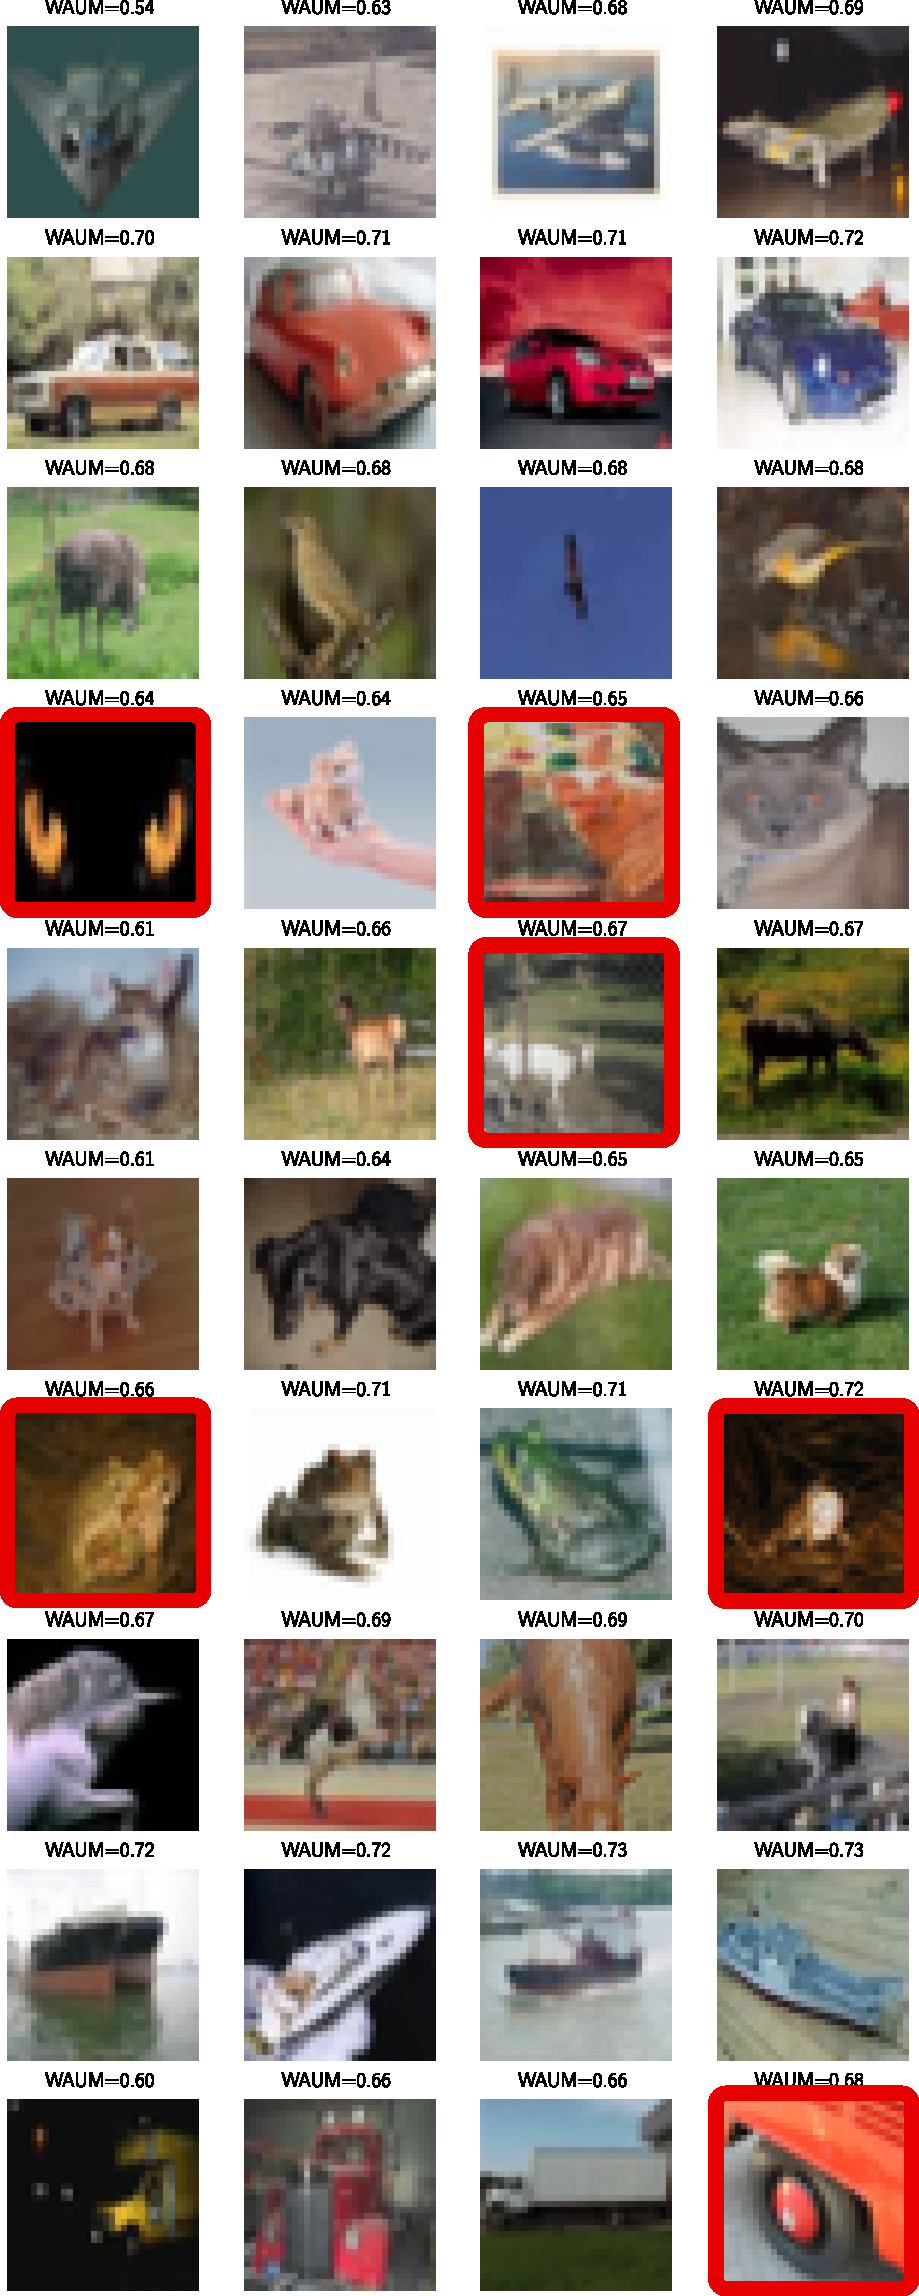
\includegraphics[width=0.3\linewidth]{images/lowest_waums_cut.pdf}}
    \hfill
    \subfloat[$\mathrm{AUMC}$ crowdsourced identification] {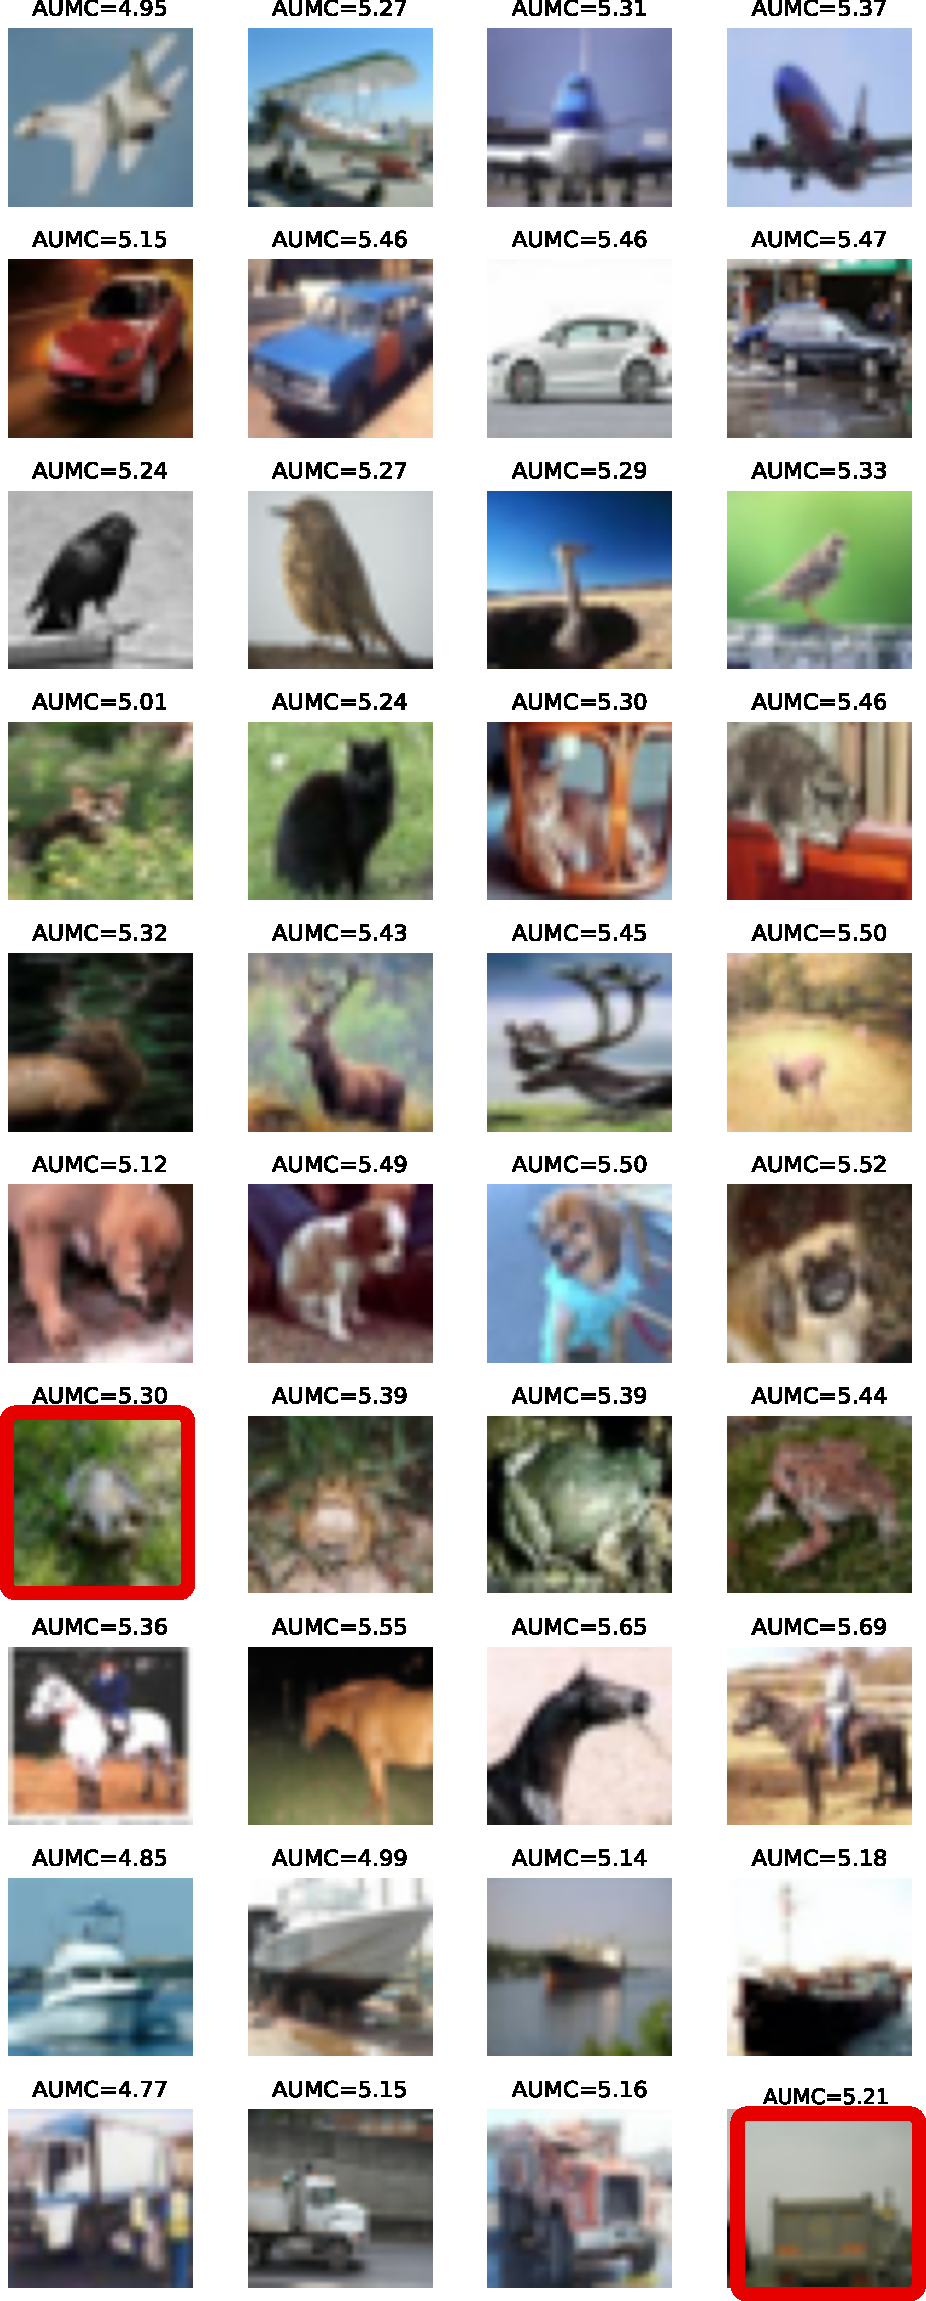
\includegraphics[width=0.3\linewidth]{images/AUMC_yang_cut.pdf}}
    \hfill
    \subfloat[$\mathrm{AUM}$ ground truth identification]{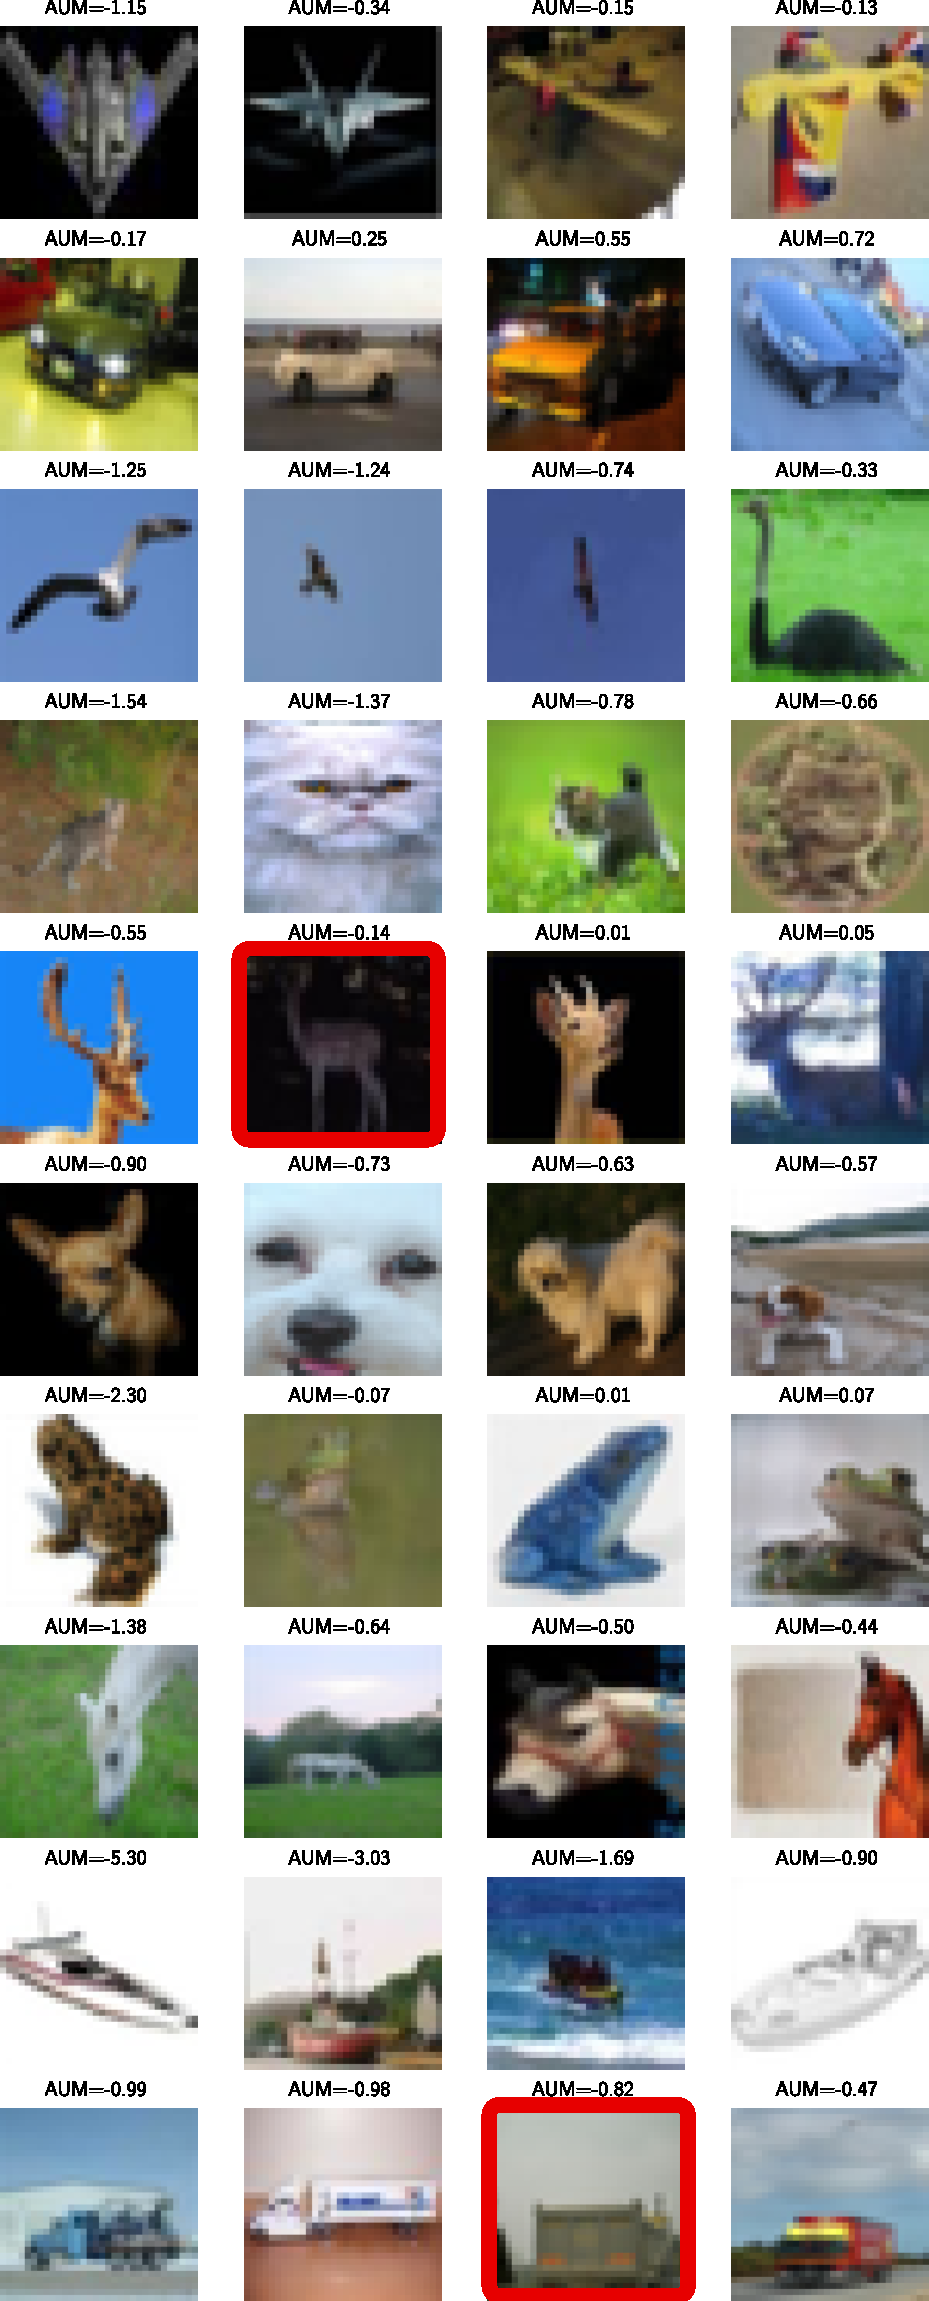
\includegraphics[width=0.3\linewidth]{images/lowest_aum_cut.pdf}}
    \caption{Comparison of the worse images detected by the $\mathrm{WAUM}$, $\mathrm{AUMC}$ and classical $\mathrm{AUM}$ preprocessing step. Identification was computed with a ResNet-18 for $50$ epochs using the parameters described in \Cref{sub:evaluation-metrics}. Each row represents the class given by the unobserved ground truth label from the \texttt{CIFAR-10} dataset. Only the $\mathrm{AUM}$ uses the ground truth label, other methods are based on the crowdsourced labels only. Images framed in red can be hard to classify.}
    \label{fig:comparison_waums_aumc}
\end{figure}


\subsubsection{Margin comparison}
\label{sec:margin_comparison}

In the $\mathrm{AUM}$, $\mathrm{AUMC}$ and $\mathrm{WAUM}$ formulae, we consider a margin from \citet{yang2020consistency} (denoted $\psi_5$ in the original article) that has better theoretical properties for top-$k$ classification but that is not the margin proposed in \citet{pleiss_identifying_2020} ($\psi_1$).
Indeed, our margin in the $\mathrm{AUM}$ is written as:
$$
\sigma_{y_i}^{(t)}(x_i) - \sigma_{[2]}^{(t)}(x_i) \enspace,
$$
instead of
$$
\sigma_{y_i}^{(t)}(x_i) - \max_{k\neq y_i}\sigma_{k}^{(t)}(x_i) \enspace.
$$
Using the \texttt{CIFAR-10H} dataset, we can compare the identified tasks using each margin.
Note that in the library used (and described in \Cref{chap:peerannot}) switching from the original margin to the top-$k$ based margin is executed with the argument \texttt{use\_pleiss=True} or \texttt{use\_pleiss=False} with the $\mathrm{WAUM}$, $\mathrm{AUM}$ and $\mathrm{AUMC}$. A comparison of the images with the lowest $\mathrm{AUM}$ is provided in \Cref{fig:aum_app_cifar}. A similar visual comparison on the \texttt{CIFAR-10H} dataset is provided in \Cref{fig:waum_app_cifar}.

\begin{figure}[thb]
    \centering
    \begin{minipage}{0.45\textwidth}
        \centering
        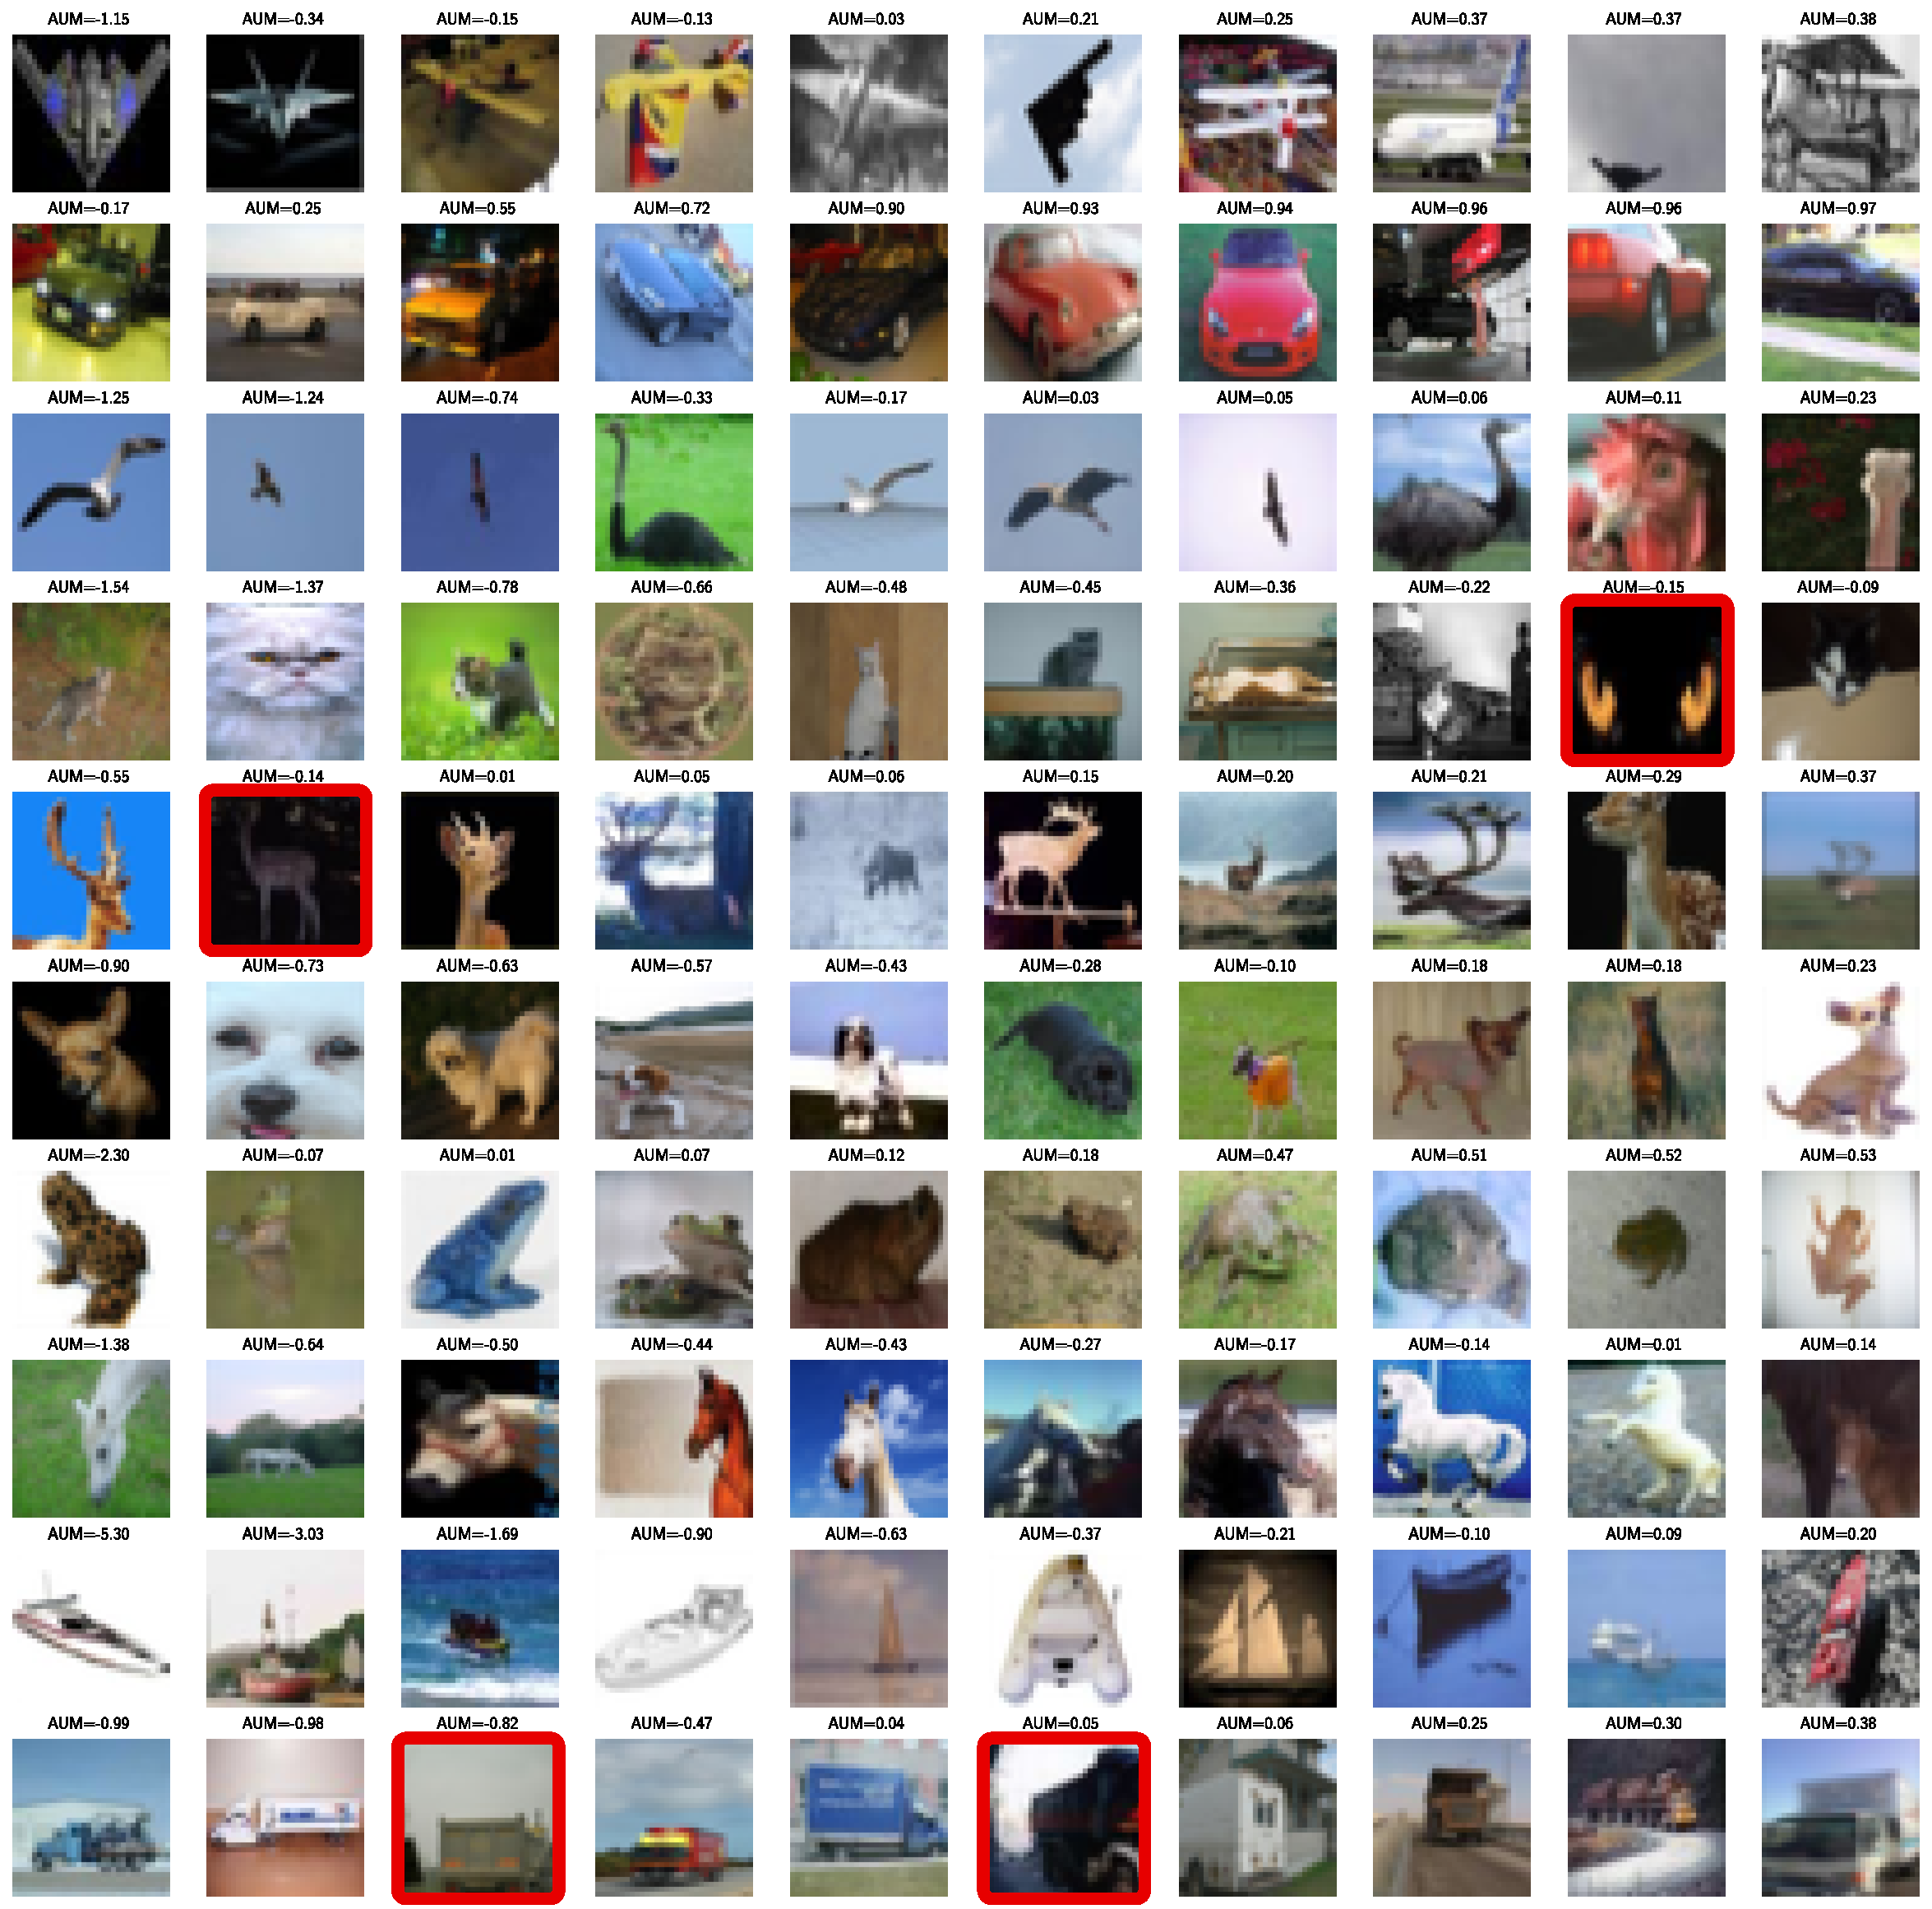
\includegraphics[width=\linewidth]{images/aum_pleiss.pdf}
        \caption{Lowest $\mathrm{AUM}$ with $\psi_1$ margin}
        \label{fig:AUM_pleiss}
    \end{minipage}
    \hfill
    \begin{minipage}{0.45\textwidth}
        \centering
        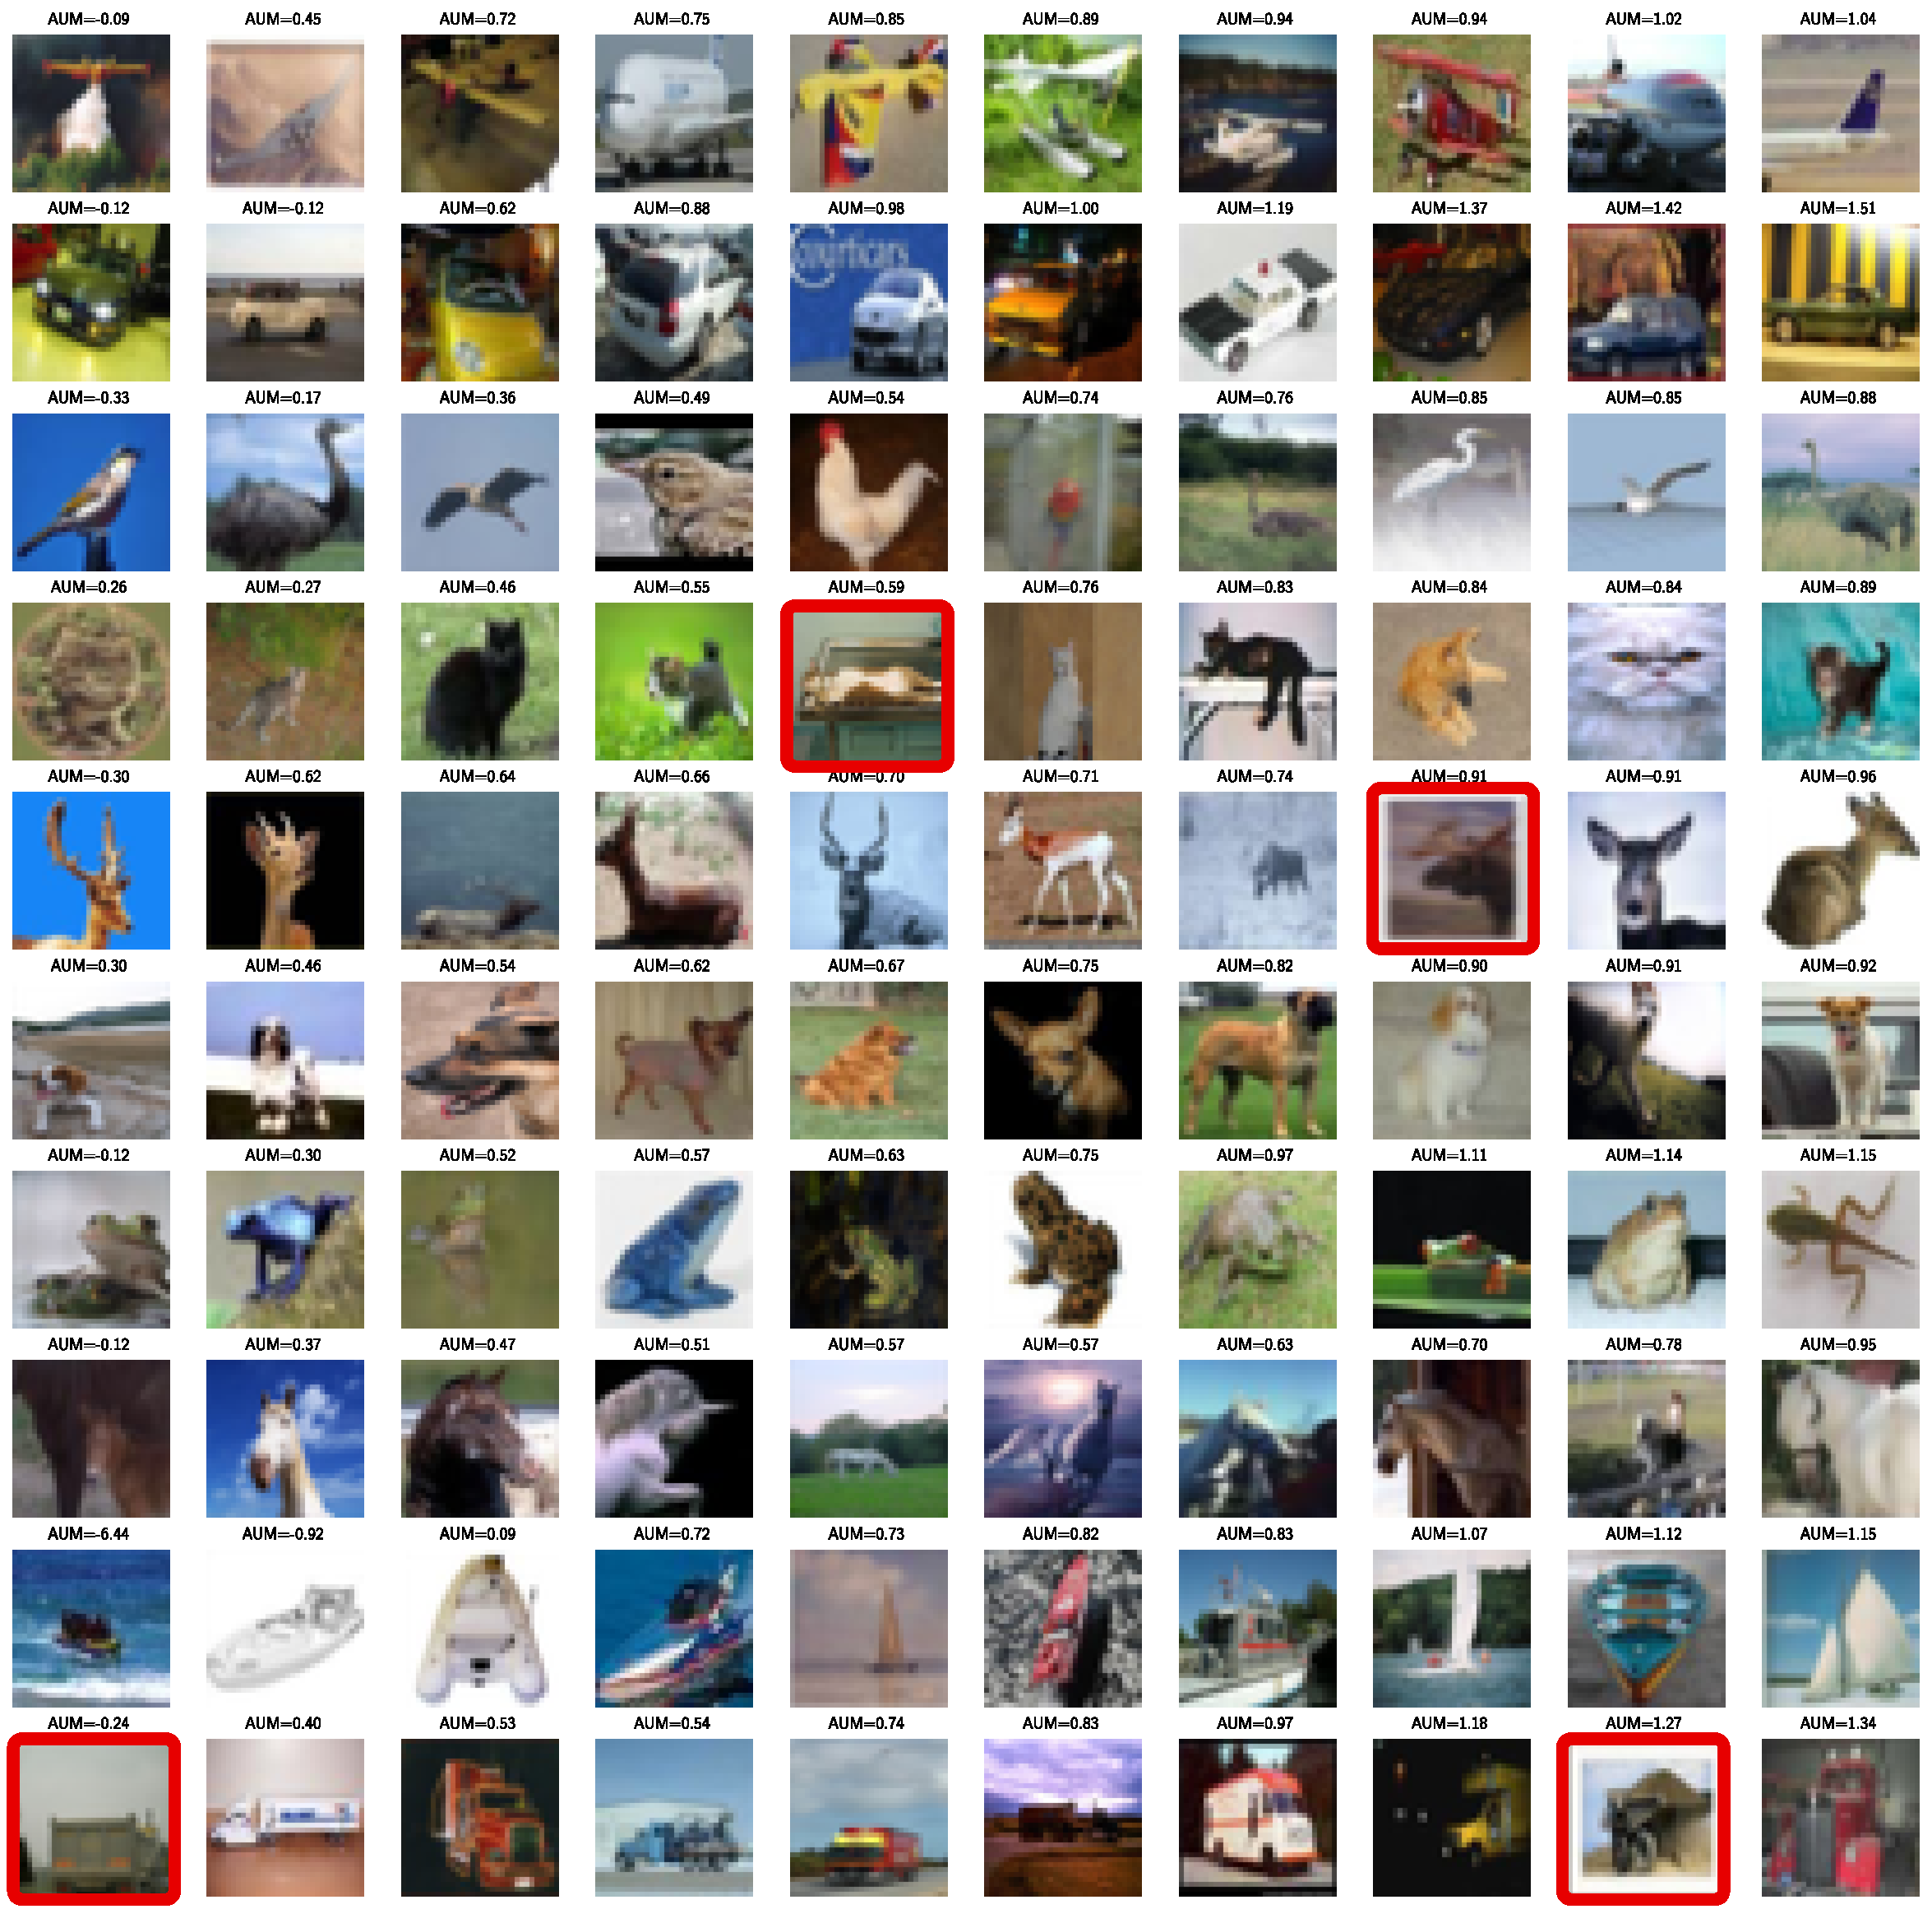
\includegraphics[width=\linewidth]{images/aum_yang.pdf}
        \caption{Lowest $\mathrm{AUM}$ with $\psi_5$ margin}
        \label{fig:AUM_yang}
    \end{minipage}
    \caption{Comparison of the images with lowest $\mathrm{AUM}$ in \texttt{CIFAR-10H} dataset using the margin from \citet{pleiss_identifying_2020} ($\psi_1$) or the margin for top-$1$ classification from \citet{yang2020consistency} ($\psi_5$). Both margins yield similar results.}
    \label{fig:aum_app_cifar}
\end{figure}

\begin{figure}[thb]
    \centering
    \begin{minipage}{0.45\textwidth}
        \centering
        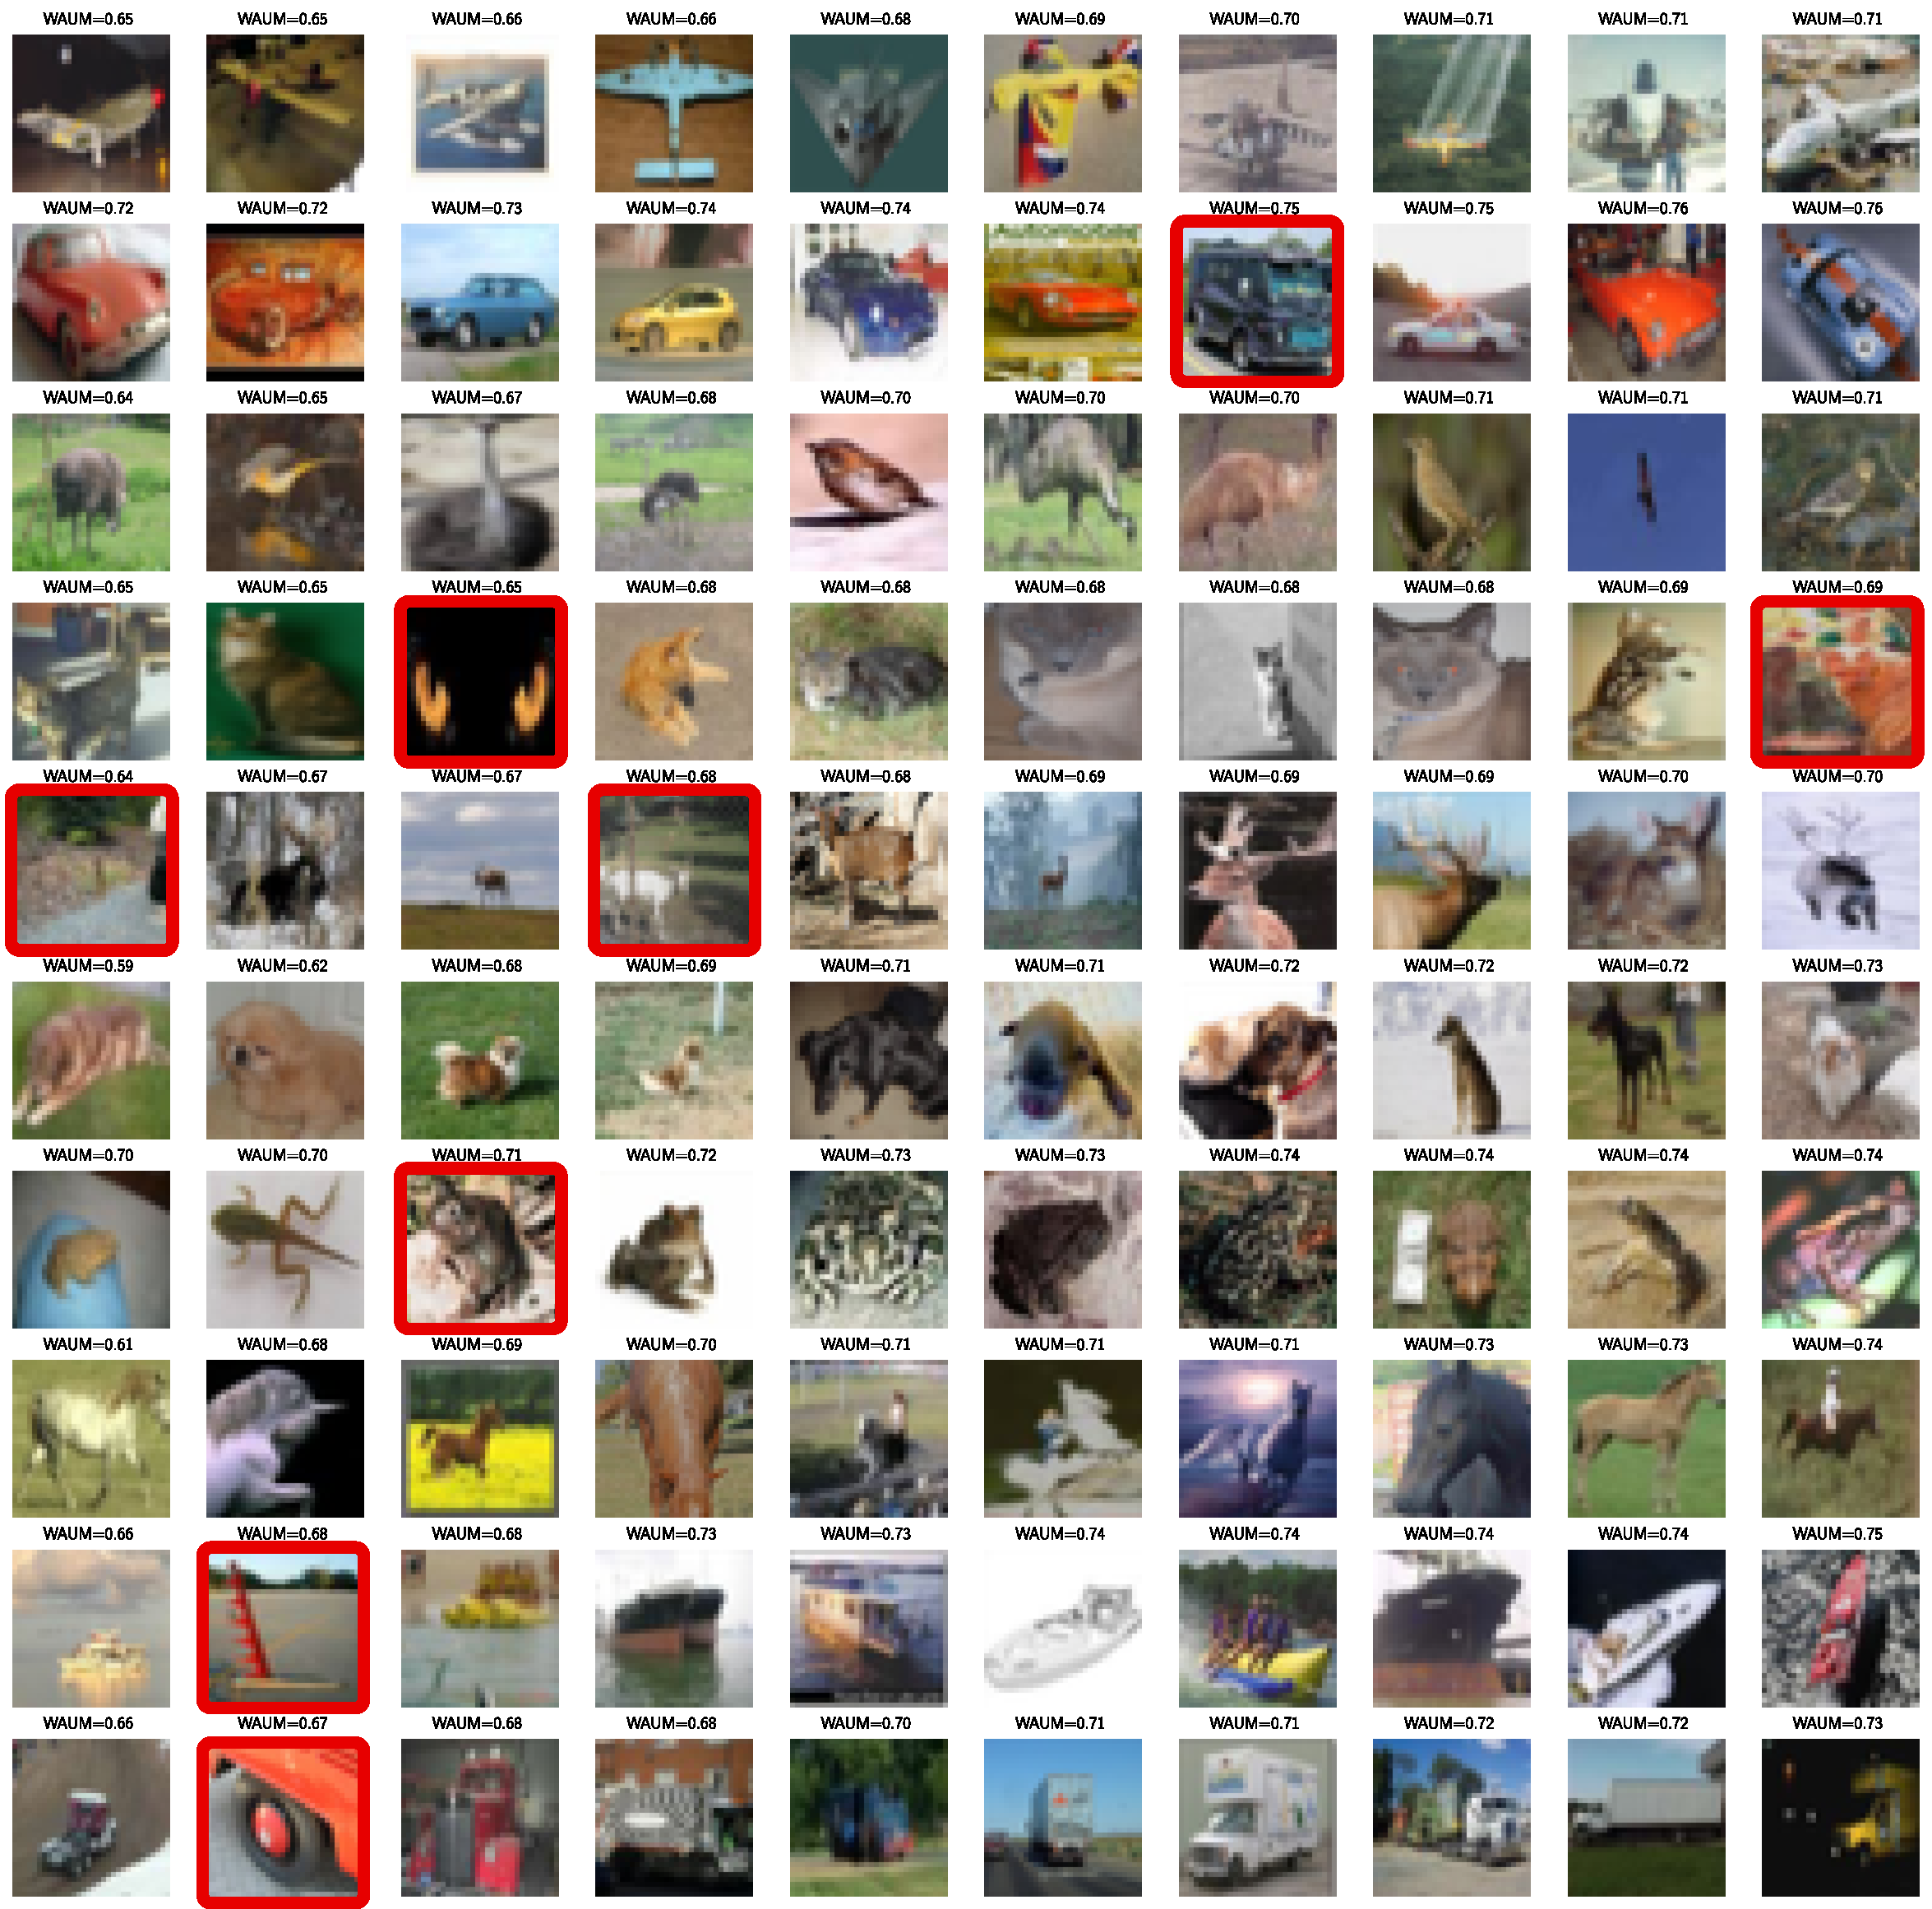
\includegraphics[width=\linewidth]{images/waum_pleiss.pdf}
        \caption{Lowest $\mathrm{WAUM}$ with $\psi_1$}
        \label{fig:WAUM_pleiss}
    \end{minipage}
    \hfill
    \begin{minipage}{0.45\textwidth}
        \centering
        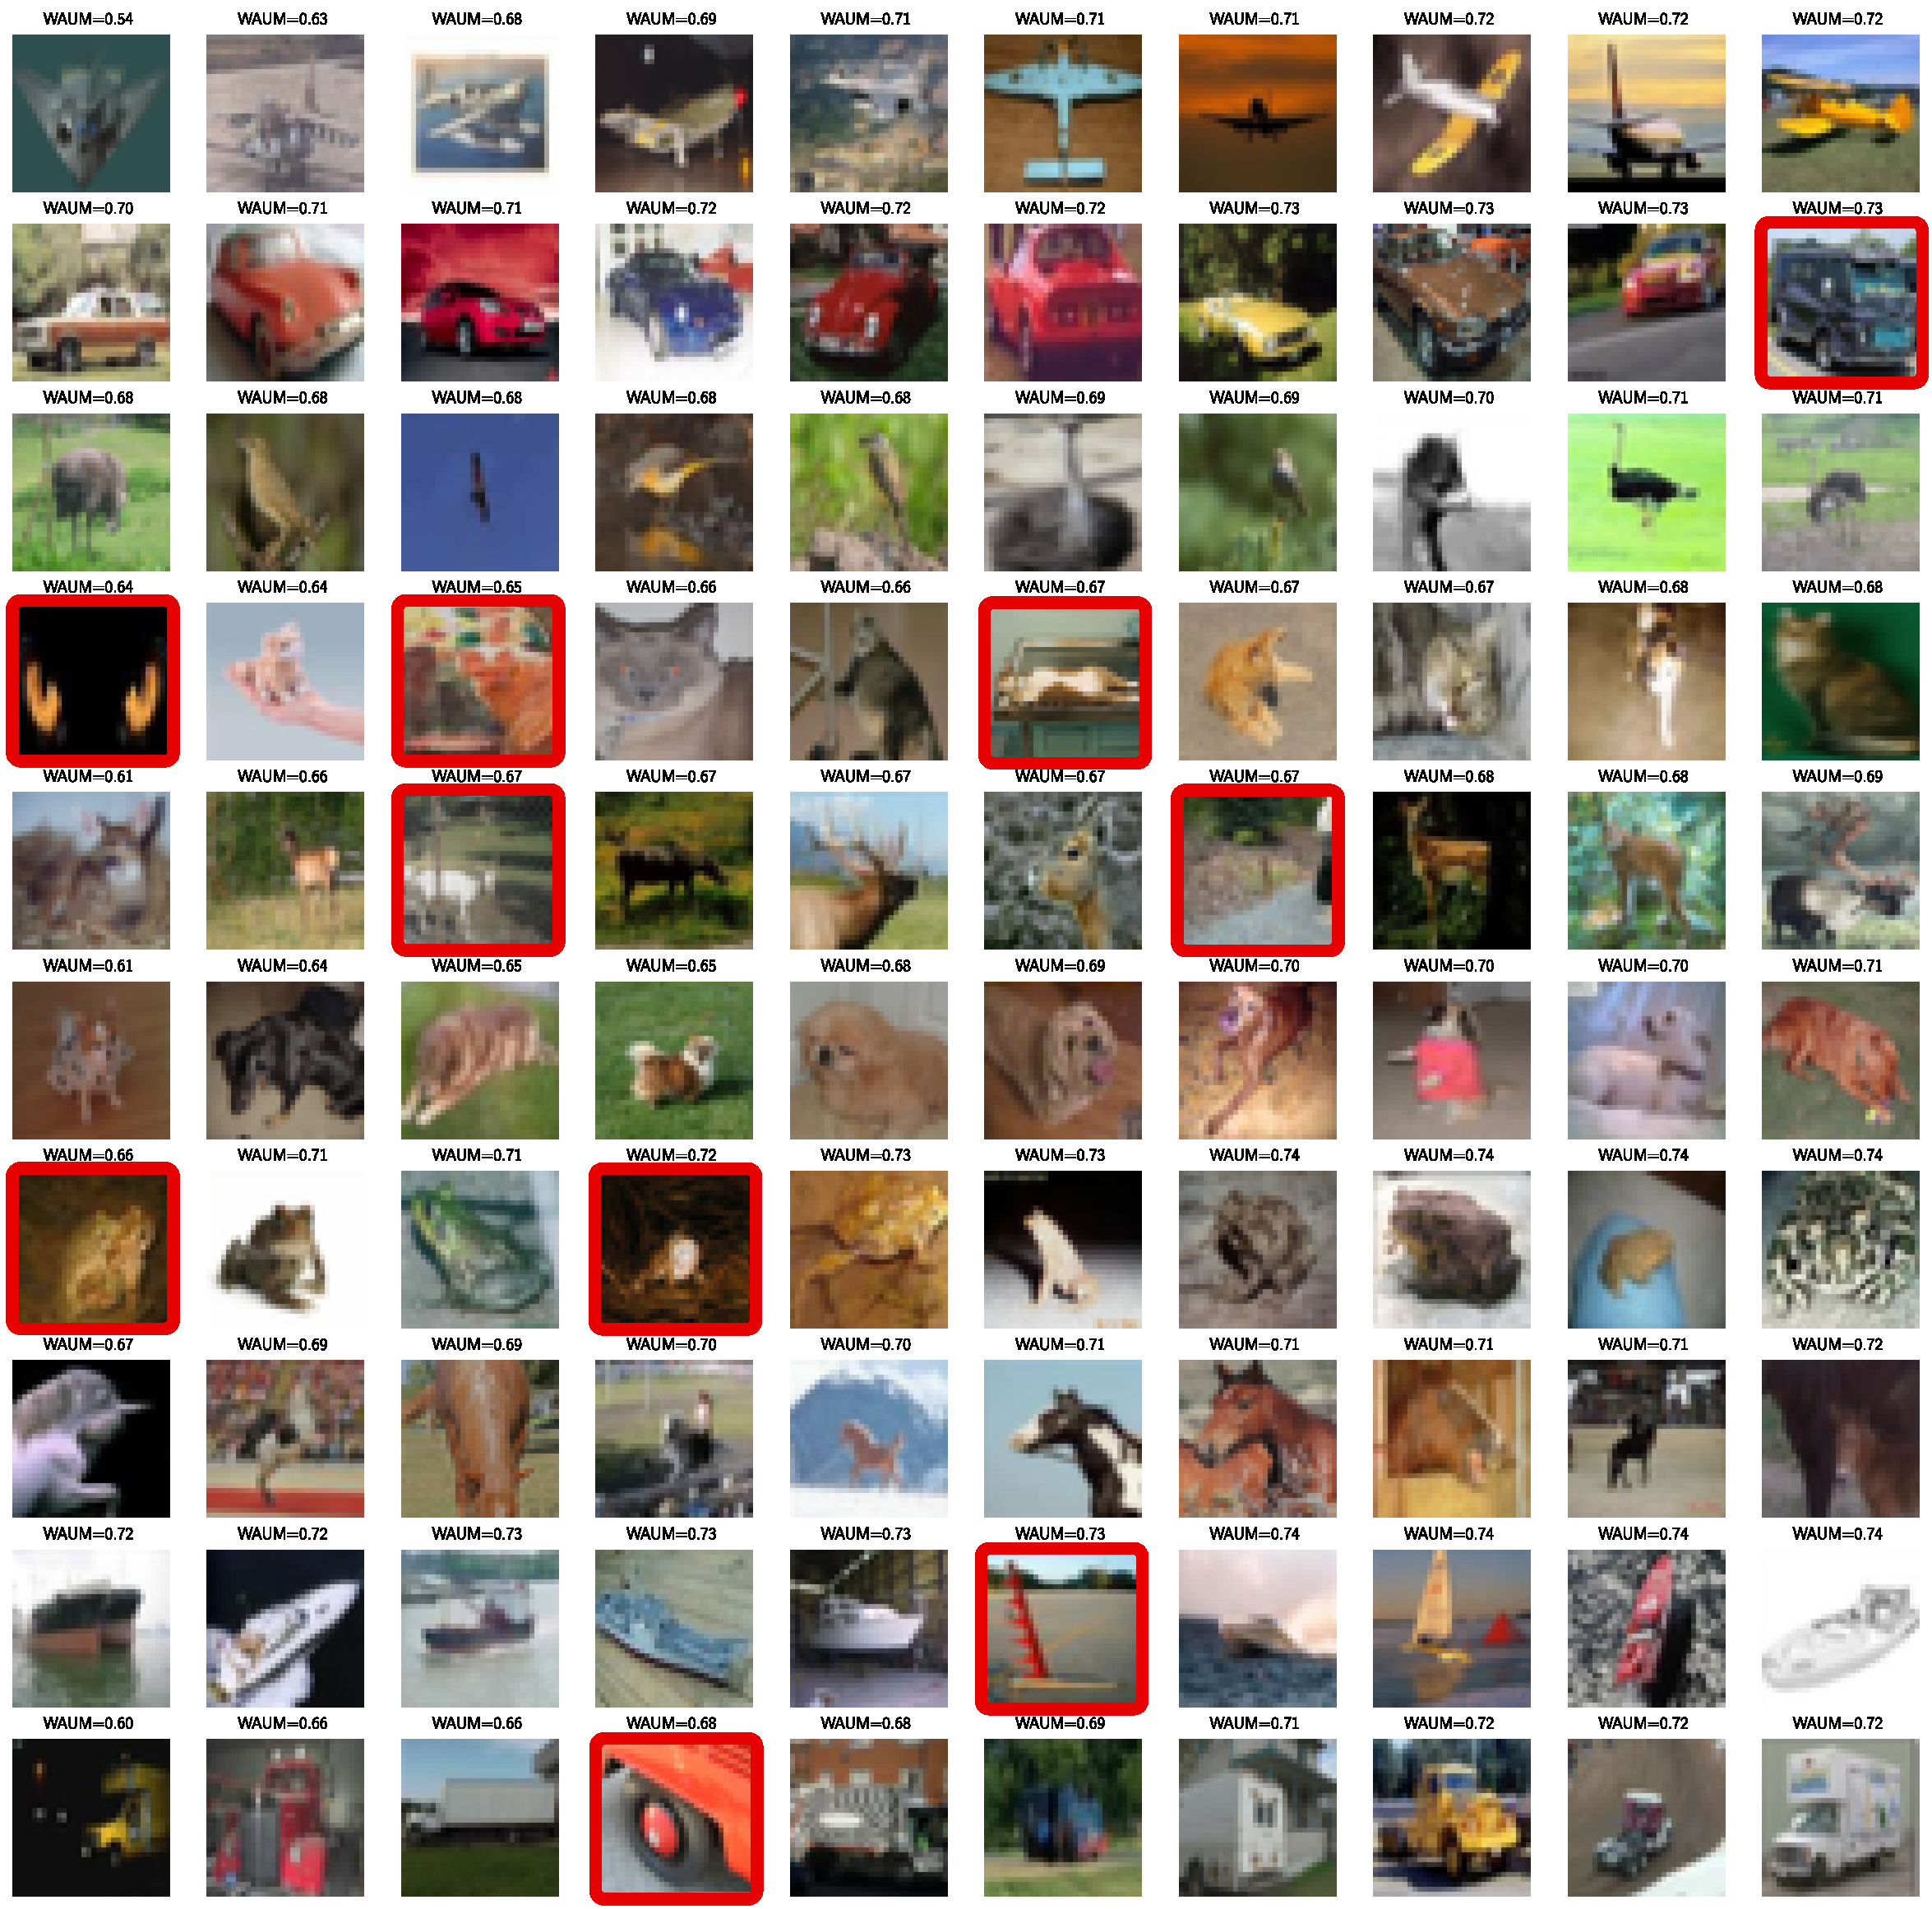
\includegraphics[width=\linewidth]{images/waum_yang.pdf}
        \caption{Lowest $\mathrm{WAUM}$ with $\psi_5$}
        \label{fig:WAUM_yang}
    \end{minipage}
    \caption{Comparison of the images with lowest $\mathrm{WAUM}$ in \texttt{CIFAR-10H} dataset using the margin from \citet{pleiss_identifying_2020} ($\psi_1$) or the margin for top-$1$ classification from \citet{yang2020consistency} ($\psi_5$). Both margins also lead to similar results.}
    \label{fig:waum_app_cifar}
\end{figure}

Furthermore, we provide an ablation study on top-$2$ accuracy scores using the $\mathrm{WAUM}$ with $\psi_1$ or $\psi_5$ margin on the \texttt{LabelMe} dataset in \Cref{tab:accuracy_comparison_top2}.
We use the cross entropy loss during the training phase.
With $\psi_5$, the top-$2$ margin writes $\sigma_{y_i}^{(t)}(x_i)- \sigma_{[3]}^{(t)}(x_i)$ as indicated in \Cref{sub:def_waum}.
We compute the top-$2$ accuracy $\emph{i.e.}$ the accuracy in recovering the true label as the first or second predicted label by the classifier.
However, note that this dataset has $K=8$ classes, hence we do not report top-$5$ accuracy as all strategies perform similarly.
We notice that performance on this dataset is similar for most strategies between the two margins used for pruning.

\begin{table}[htbp]
    \centering
    \caption{Top-$2$ Accuracy comparison on the \texttt{LabelMe} dataset using the modified VGG-16 backbone and the same hyperparameters as in \Cref{subsec:evaluate}. Results are averaged over $5$ repetitions, and errors are standard deviations.
    }
    \begin{tabular}{lccc}
        \textbf{Strategy} & \textbf{Top-2 no pruning} & \textbf{Top-2 WAUM($\psi_1$)} & \textbf{Top-2 WAUM($\psi_5$)} \\
        \hline
        MV   & $91.25 \pm 2.01$ & $91.17 \pm 2.12$ & $92.02 \pm 2.08 $ \\
        NS   & $90.92 \pm 1.53$ & $90.41 \pm 2.77$ & $89.91 \pm 1.08$ \\
        DS   & $89.98 \pm 1.12$ & $90.24 \pm 0.92$ & $91.41\pm 0.99$ \\
        GLAD & $90.78 \pm 0.98$ & $91.34 \pm 1.59$ & $90.49 \pm 0.38$ \\
        WDS  & $89.56 \pm 1.76 $ & $90.82 \pm 1.81$ & $91.16 \pm 2.78$ \\
        CrowdLayer & $87.45 \pm 2.03$ & $88.33 \pm 1.49$ & $88.57 \pm 2.51$ \\
        CoNAL($\lambda=0$) & $92.34 \pm 0.74$ & $89.49 \pm 0.53$ & $94.30 \pm 1.32$ \\
        CoNAL($\lambda=10^{-4}$) & $91.68 \pm 1.01$ & $94.10  \pm 0.9$ & $94.93 \pm 0.76$\\
    \end{tabular}
    \label{tab:accuracy_comparison_top2}
\end{table}

\subsubsection{Limitations and assumptions}
First, concerning the weights $s_i^{(j)}$ (reflecting the trust in the image/worker interaction), we rely on confusion matrices $\{\hat{\pi}^{(j)}\}_{j\in [n_\texttt{worker}]}$.
The DS model \citep{dawid_maximum_1979} can be naturally used to estimate such matrices $\pi^{(j)}\in\mathbb{R}^{K\times K}$ for each worker $w_j$.
Yet, the quadratic number of parameters (w.r.t. $K$) to be estimated for each worker can create convergence issues for the vanilla DS model when $K$ is large.
But as stated in \Cref{sub:def_waum}, any model that can estimate confusion matrices can be considered for the $\mathrm{WAUM}$'s computation.
We detail below some possible variants, that could help compute the confusion matrices used in the $\mathrm{WAUM}$ for the trust score computation.
\begin{itemize}
    \item \citet{sinha2018fast} accelerated the vanilla DS by constraining the estimated labels' distribution to be a Dirac mass. Hence, predicted labels are hard labels. This leads to worse calibration errors than vanilla DS but preserves the same accuracy.
    \item \citet{passonneau-carpenter-2014-benefits} introduced Dirichlet priors on the confusion matrices' rows and the prevalence $\rho$ to incorporate previously known information on the workers in the model (from other experiments).
    \item \citet{servajean2017crowdsourcing} exploited the sparsity of the confusion matrices to cope with a large $K$.
    \item \citet{imamura2018analysis} estimated with variational inference $L \ll n_{\texttt{worker}}$ clusters of workers, constraining at most $L$ different confusion matrices. This reduces the number of parameters required  from $K^2\times n_{\texttt{worker}}$ to $K^2\times L$.
\end{itemize}

\paragraph{Pruning and \emph{i.i.d} assumption.} The pruning at preprocessing can induce a distortion in the training data distribution.
A usual assumption made on learning problems is that the task/label pairs are \emph{i.i.d}.
However, by removing some of the hardest tasks, the new dataset $\mathcal{D}_{\text{pruned}}$ contains tasks that are not independent anymore.
We should also keep in mind that \citet{ilyas2022datamodels} have shown that in the standard datasets, the data is not \emph{i.i.d} to begin with.

\section{Conclusion}
In this chapter, we investigate crowdsourcing aggregation models and how judging systems may impact generalization performance.
Most models consider the ambiguity from the workers' perspective (very few consider the difficulty of the task itself) and evaluate workers on hard tasks that might be too ambiguous to be relevant, leading to a performance drop.
Using a popular model (DS), we develop the $\mathrm{WAUM}$, a flexible feature-aware metric that can identify hard tasks and improves generalization performance over vanilla strategies and naive pruning $\mathrm{AUMC}$ that both extend the existing $\mathrm{AUM}$ to the crowdsourcing setting.
It also yields a fair evaluation of workers' abilities and supports recent research on data pruning in supervised datasets.
Independently of pruning, the $\mathrm{WAUM}$ allows identifying early the images that need extra labeling efforts or that are impossible to correctly label.

Extension of the $\mathrm{WAUM}$ to more general learning tasks (\emph{e.g} top-$k$ classification, \Cref{sec:margin_comparison}) would be natural, including sequential label.
Indeed, the $\mathrm{WAUM}$ could help to identify tasks requiring additional expertise and guide how to allocate more experts/workers for such identified tasks. However, there is a community need for openly available datasets with both tasks and votes for such evaluation.

\paragraph*{Broader Impact Statement.}
As this work proposes a method to prune tasks from training datasets based on human-derived data, we remind that pruning based on learning difficulty can induce a learning bias for the model.
To mitigate this, only pruning a small portion of the dataset can help avoid any class with a small number of representatives to be removed of the dataset.
Also, in this paper, we only remove tasks that are difficult to classify, we do not remove workers from the dataset.
In particular, there is no repercussion on their pay, and by only evaluating them on tasks that are not detected as ambiguous, we evaluate their abilities on fairer tasks.

